%%=============================================================================
%% LaTeX sjabloon voor bachelorproef, HoGent Bedrijf en Organisatie
%% Opleiding Toegepaste Informatica
%%=============================================================================

\documentclass[fleqn,a4paper,12pt]{book}

%%=============================================================================
%% LaTeX sjabloon voor de bachelorproef, HoGent Bedrijf en Organisatie
%% Opleiding toegepaste informatica
%%
%% Structuur en algemene vormgeving. Meestal hoef je hier niets te wijzigen.
%%
%% Vormgeving gebaseerd op "The Legrand Orange Book", version 2.0 (9/2/15)
%% door Mathias Legrand (legrand.mathias@gmail.com) met aanpassingen door
%% Vel (vel@latextemplates.com). Het oorspronkelijke template is te vinden op
%% http://www.LaTeXTemplates.com
%%
%% Aanpassingen voor HoGent toegepaste informatica: 
%%   Bert Van Vreckem <bert.vanvreckem@hogent.be>
%% Licentie: 
%%   CC BY-NC-SA 3.0 (http://creativecommons.org/licenses/by-nc-sa/3.0/)
%%=============================================================================

%%-----------------------------------------------------------------------------
%% Packages
%%-----------------------------------------------------------------------------

\usepackage[top=3cm,bottom=3cm,left=3cm,right=3cm,headsep=10pt,a4paper]{geometry} % Page margins
\usepackage[utf8]{inputenc}  % Accenten gebruiken in tekst (vb. é ipv \'e)
\usepackage{amsfonts}        % AMS math packages: extra wiskundige
\usepackage{amsmath}         %   symbolen (o.a. getallen-
\usepackage{amssymb}         %   verzamelingen N, R, Z, Q, etc.)
\usepackage[english,dutch]{babel}    % Taalinstellingen: woordsplitsingen,
                             %  commando's voor speciale karakters
                             %  ("dutch" voor NL)
\usepackage{iflang}
\usepackage{eurosym}         % Euro-symbool €
\usepackage{geometry}
\usepackage{graphicx}        % Invoegen van tekeningen
\graphicspath{{img/}}       % Specifies the directory where pictures are stored
\usepackage{tikz}            % Required for drawing custom shapes
\usepackage[pdftex,bookmarks=true]{hyperref}
                             % PDF krijgt klikbare links & verwijzingen,
                             %  inhoudstafel
\usepackage{enumitem}        % Customize lists
\setlist{nolistsep}         % Reduce spacing between list items
\usepackage{listings}        % Broncode mooi opmaken
\usepackage{multirow}        % Tekst over verschillende cellen in tabellen
\usepackage{rotating}        % Tabellen en figuren roteren

\usepackage{booktabs}        % Required for nicer horizontal rules in tables

\usepackage{xcolor}          % Required for specifying colors by name
\definecolor{maincolor}{RGB}{0,147,208} % Define the main color used for 
                             % highlighting throughout the book
                             % 0, 147, 208 = officiële kleur HoGent FBO

% Paragraph style: no indent, add space between paragraphs
\setlength{\parindent}{0em}
\setlength{\parskip}{1em}

\usepackage{etoolbox}
\usepackage{titling} % Macros for title, author, etc
\usepackage{lipsum}          % Voor vultekst (lorem ipsum)

%----------------------------------------------------------------------------------------
%	FONTS
%----------------------------------------------------------------------------------------

\usepackage{avant} % Use the Avantgarde font for headings
%\usepackage{times} % Use the Times font for headings
\usepackage{mathptmx} % Use the Adobe Times Roman as the default text font together with math symbols from the Sym­bol, Chancery and Com­puter Modern fonts

\usepackage{microtype} % Slightly tweak font spacing for aesthetics
\usepackage[utf8]{inputenc} % Required for including letters with accents
\usepackage[T1]{fontenc} % Use 8-bit encoding that has 256 glyphs

%------------------------------------------------------------------------------
%	TITLE PAGE
%------------------------------------------------------------------------------
\lstset{
	breaklines=true,
	breakatwhitespace=true,
}

\newcommand{\inserttitlepage}{%
\begin{titlepage}
  \newgeometry{top=2cm,bottom=1.5cm,left=1.5cm,right=1.5cm}
  \begin{center}

    \begingroup
    \rmfamily
    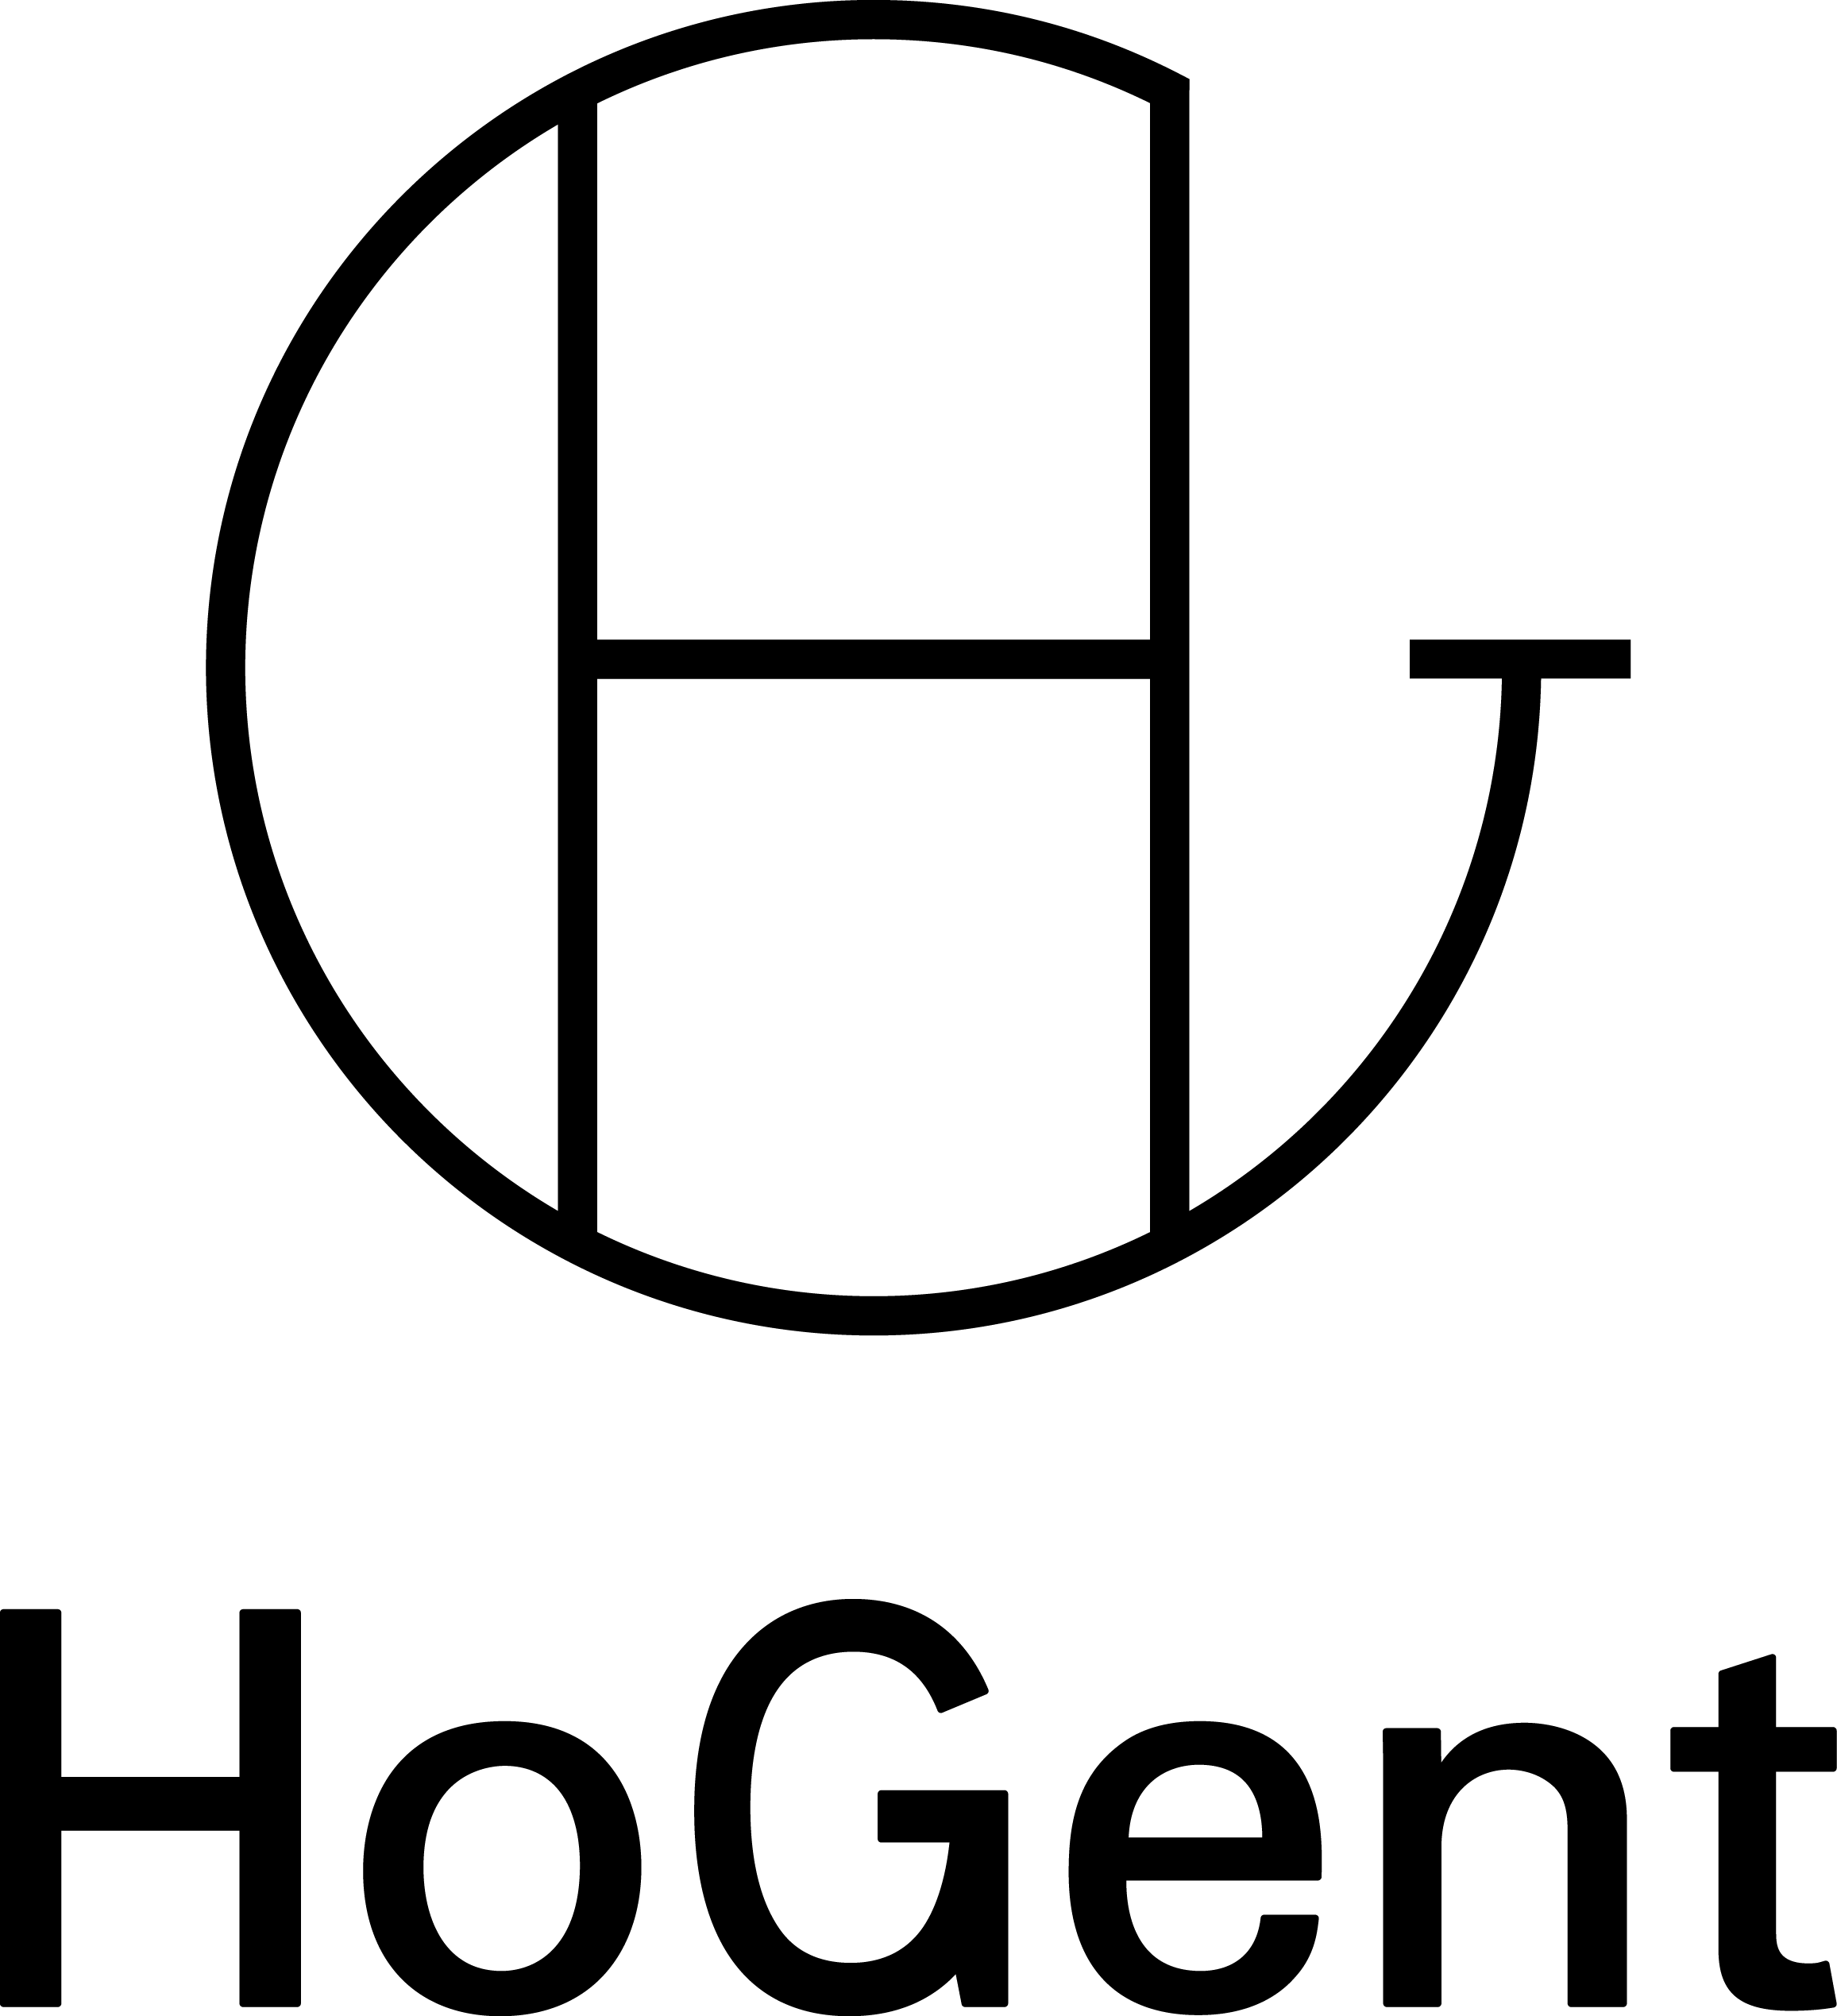
\includegraphics[width=2.5cm]{img/HG-beeldmerk-woordmerk}\\[.5cm]
    Faculteit Bedrijf en Organisatie\\[3cm]
    \titel
    \vfill
    \student\\[3.5cm]
    Scriptie voorgedragen tot het bekomen van de graad van\\professionele bachelor in de toegepaste informatica\\[2cm]
    Promotor:\\
    \promotor\\
    \ifdefempty{\copromotor}{\vspace{2.5cm}}{Co-promotor:\\\copromotor\\[2.5cm]}
    Instelling: \instelling\\[.5cm]
    Academiejaar: \academiejaar\\[.5cm]
    \ifcase \examenperiode \or Eerste \or Tweede \else Derde \fi examenperiode
    \endgroup

  \end{center}
  \restoregeometry
\end{titlepage}
  \emptypage
\begin{titlepage}
  \newgeometry{top=5.35cm,bottom=1.5cm,left=1.5cm,right=1.5cm}
  \begin{center}

    \begingroup
    \rmfamily
    \IfLanguageName{dutch}{Faculteit Bedrijf en Organisatie}{Faculty of Business and Information Management}\\[3cm]
    \titel
    \vfill
    \student\\[3.5cm]
    \IfLanguageName{dutch}{Scriptie voorgedragen tot het bekomen van de graad van\\professionele bachelor in de toegepaste informatica}{Thesis submitted in partial fulfilment of the requirements for the degree of\\professional bachelor of applied computer science}\\[2cm]
    Promotor:\\
    \promotor\\
    \ifdefempty{\copromotor}{\vspace{2.5cm}}{Co-promotor:\\\copromotor\\[2.5cm]}
    \IfLanguageName{dutch}{Instelling}{Institution}: \instelling\\[.5cm]
    \IfLanguageName{dutch}{Academiejaar}{Academic year}: \academiejaar\\[.5cm]
    \IfLanguageName{dutch}{%
    \ifcase \examenperiode \or Eerste \or Tweede \else Derde \fi examenperiode}{%
    \ifcase \examenperiode \or First \or Second \else Third \fi examination period}
    \endgroup

  \end{center}
  \restoregeometry
\end{titlepage}
}

%----------------------------------------------------------------------------------------
%	BIBLIOGRAPHY AND INDEX
%----------------------------------------------------------------------------------------

\usepackage[style=apa,backend=biber]{biblatex}
\usepackage{csquotes}
\DeclareLanguageMapping{dutch}{dutch-apa}
\addbibresource{bachproef-tin.bib} % BibTeX bibliography file
\addbibresource{voorstel/biblio.bib}
\defbibheading{bibempty}{}

\usepackage{calc} % For simpler calculation - used for spacing the index letter headings correctly
\usepackage{makeidx} % Required to make an index
\makeindex % Tells LaTeX to create the files required for indexing

%----------------------------------------------------------------------------------------
%	MAIN TABLE OF CONTENTS
%----------------------------------------------------------------------------------------

\usepackage{titletoc} % Required for manipulating the table of contents

\contentsmargin{0cm} % Removes the default margin

% Part text styling
\titlecontents{part}[0cm]
{\addvspace{20pt}\centering\large\bfseries}
{}
{}
{}

% Chapter text styling
\titlecontents{chapter}[1.25cm] % Indentation
{\addvspace{12pt}\large\sffamily\bfseries} % Spacing and font options for chapters
{\color{maincolor!60}\contentslabel[\Large\thecontentslabel]{1.25cm}\color{maincolor}} % Chapter number
{\color{maincolor}}
{\color{maincolor!60}\normalsize\;\titlerule*[.5pc]{.}\;\thecontentspage} % Page number

% Section text styling
\titlecontents{section}[1.25cm] % Indentation
{\addvspace{3pt}\sffamily\bfseries} % Spacing and font options for sections
{\contentslabel[\thecontentslabel]{1.25cm}} % Section number
{}
{\hfill\color{black}\thecontentspage} % Page number
[]

% Subsection text styling
\titlecontents{subsection}[1.25cm] % Indentation
{\addvspace{1pt}\sffamily\small} % Spacing and font options for subsections
{\contentslabel[\thecontentslabel]{1.25cm}} % Subsection number
{}
{\ \titlerule*[.5pc]{.}\;\thecontentspage} % Page number
[]

% List of figures
\titlecontents{figure}[0em]
{\addvspace{-5pt}\sffamily}
{\thecontentslabel\hspace*{1em}}
{}
{\ \titlerule*[.5pc]{.}\;\thecontentspage}
[]

% List of tables
\titlecontents{table}[0em]
{\addvspace{-5pt}\sffamily}
{\thecontentslabel\hspace*{1em}}
{}
{\ \titlerule*[.5pc]{.}\;\thecontentspage}
[]

%----------------------------------------------------------------------------------------
%	MINI TABLE OF CONTENTS IN PART HEADS
%----------------------------------------------------------------------------------------

% Chapter text styling
\titlecontents{lchapter}[0em] % Indenting
{\addvspace{15pt}\large\sffamily\bfseries} % Spacing and font options for chapters
{\color{maincolor}\contentslabel[\Large\thecontentslabel]{1.25cm}\color{maincolor}} % Chapter number
{}
{\color{maincolor}\normalsize\sffamily\bfseries\;\titlerule*[.5pc]{.}\;\thecontentspage} % Page number

% Section text styling
\titlecontents{lsection}[0em] % Indenting
{\sffamily\small} % Spacing and font options for sections
{\contentslabel[\thecontentslabel]{1.25cm}} % Section number
{}
{}

% Subsection text styling
\titlecontents{lsubsection}[.5em] % Indentation
{\normalfont\footnotesize\sffamily} % Font settings
{}
{}
{}

%----------------------------------------------------------------------------------------
%	PAGE HEADERS
%----------------------------------------------------------------------------------------

\usepackage{fancyhdr} % Required for header and footer configuration

\pagestyle{fancy}
\renewcommand{\chaptermark}[1]{\markboth{\sffamily\normalsize\bfseries\chaptername\ \thechapter.\ #1}{}} % Chapter text font settings
\renewcommand{\sectionmark}[1]{\markright{\sffamily\normalsize\thesection\hspace{5pt}#1}{}} % Section text font settings
\fancyhf{} \fancyhead[LE,RO]{\sffamily\normalsize\thepage} % Font setting for the page number in the header
\fancyhead[LO]{\rightmark} % Print the nearest section name on the left side of odd pages
\fancyhead[RE]{\leftmark} % Print the current chapter name on the right side of even pages
\renewcommand{\headrulewidth}{0.5pt} % Width of the rule under the header
\addtolength{\headheight}{2.5pt} % Increase the spacing around the header slightly
\renewcommand{\footrulewidth}{0pt} % Removes the rule in the footer
\fancypagestyle{plain}{\fancyhead{}\renewcommand{\headrulewidth}{0pt}} % Style for when a plain pagestyle is specified

% Removes the header from odd empty pages at the end of chapters
\makeatletter
\renewcommand{\cleardoublepage}{
\clearpage\ifodd\c@page\else
\hbox{}
\vspace*{\fill}
\thispagestyle{empty}
\newpage
\fi}

%----------------------------------------------------------------------------------------
%	THEOREM STYLES
%----------------------------------------------------------------------------------------

\usepackage{amsmath,amsfonts,amssymb,amsthm} % For math equations, theorems, symbols, etc

\newcommand{\intoo}[2]{\mathopen{]}#1\,;#2\mathclose{[}}
\newcommand{\ud}{\mathop{\mathrm{{}d}}\mathopen{}}
\newcommand{\intff}[2]{\mathopen{[}#1\,;#2\mathclose{]}}
\newtheorem{notation}{Notation}[chapter]

% Boxed/framed environments
\newtheoremstyle{maincolornumbox}% % Theorem style name
{0pt}% Space above
{0pt}% Space below
{\normalfont}% % Body font
{}% Indent amount
{\small\bf\sffamily\color{maincolor}}% % Theorem head font
{\;}% Punctuation after theorem head
{0.25em}% Space after theorem head
{\small\sffamily\color{maincolor}\thmname{#1}\nobreakspace\thmnumber{\@ifnotempty{#1}{}\@upn{#2}}% Theorem text (e.g. Theorem 2.1)
\thmnote{\nobreakspace\the\thm@notefont\sffamily\bfseries\color{black}---\nobreakspace#3.}} % Optional theorem note
\renewcommand{\qedsymbol}{$\blacksquare$}% Optional qed square

\newtheoremstyle{blacknumex}% Theorem style name
{5pt}% Space above
{5pt}% Space below
{\normalfont}% Body font
{} % Indent amount
{\small\bf\sffamily}% Theorem head font
{\;}% Punctuation after theorem head
{0.25em}% Space after theorem head
{\small\sffamily{\tiny\ensuremath{\blacksquare}}\nobreakspace\thmname{#1}\nobreakspace\thmnumber{\@ifnotempty{#1}{}\@upn{#2}}% Theorem text (e.g. Theorem 2.1)
\thmnote{\nobreakspace\the\thm@notefont\sffamily\bfseries---\nobreakspace#3.}}% Optional theorem note

\newtheoremstyle{blacknumbox} % Theorem style name
{0pt}% Space above
{0pt}% Space below
{\normalfont}% Body font
{}% Indent amount
{\small\bf\sffamily}% Theorem head font
{\;}% Punctuation after theorem head
{0.25em}% Space after theorem head
{\small\sffamily\thmname{#1}\nobreakspace\thmnumber{\@ifnotempty{#1}{}\@upn{#2}}% Theorem text (e.g. Theorem 2.1)
\thmnote{\nobreakspace\the\thm@notefont\sffamily\bfseries---\nobreakspace#3.}}% Optional theorem note

% Non-boxed/non-framed environments
\newtheoremstyle{maincolornum}% % Theorem style name
{5pt}% Space above
{5pt}% Space below
{\normalfont}% % Body font
{}% Indent amount
{\small\bf\sffamily\color{maincolor}}% % Theorem head font
{\;}% Punctuation after theorem head
{0.25em}% Space after theorem head
{\small\sffamily\color{maincolor}\thmname{#1}\nobreakspace\thmnumber{\@ifnotempty{#1}{}\@upn{#2}}% Theorem text (e.g. Theorem 2.1)
\thmnote{\nobreakspace\the\thm@notefont\sffamily\bfseries\color{black}---\nobreakspace#3.}} % Optional theorem note
\renewcommand{\qedsymbol}{$\blacksquare$}% Optional qed square
\makeatother

% Defines the theorem text style for each type of theorem to one of the three styles above
\newcounter{dummy}
\numberwithin{dummy}{section}
\theoremstyle{maincolornumbox}
\newtheorem{theoremeT}[dummy]{Theorem}
\newtheorem{problem}{Problem}[chapter]
\newtheorem{exerciseT}{Exercise}[chapter]
\theoremstyle{blacknumex}
\newtheorem{exampleT}{Example}[chapter]
\theoremstyle{blacknumbox}
\newtheorem{vocabulary}{Vocabulary}[chapter]
\newtheorem{definitionT}{Definition}[section]
\newtheorem{corollaryT}[dummy]{Corollary}
\theoremstyle{maincolornum}
\newtheorem{proposition}[dummy]{Proposition}

%----------------------------------------------------------------------------------------
%	DEFINITION OF COLORED BOXES
%----------------------------------------------------------------------------------------

\RequirePackage[framemethod=default]{mdframed} % Required for creating the theorem, definition, exercise and corollary boxes

% Theorem box
\newmdenv[skipabove=7pt,
skipbelow=7pt,
backgroundcolor=black!5,
linecolor=maincolor,
innerleftmargin=5pt,
innerrightmargin=5pt,
innertopmargin=5pt,
leftmargin=0cm,
rightmargin=0cm,
innerbottommargin=5pt]{tBox}

% Exercise box
\newmdenv[skipabove=7pt,
skipbelow=7pt,
rightline=false,
leftline=true,
topline=false,
bottomline=false,
backgroundcolor=maincolor!10,
linecolor=maincolor,
innerleftmargin=5pt,
innerrightmargin=5pt,
innertopmargin=5pt,
innerbottommargin=5pt,
leftmargin=0cm,
rightmargin=0cm,
linewidth=4pt]{eBox}

% Definition box
\newmdenv[skipabove=7pt,
skipbelow=7pt,
rightline=false,
leftline=true,
topline=false,
bottomline=false,
linecolor=maincolor,
innerleftmargin=5pt,
innerrightmargin=5pt,
innertopmargin=0pt,
leftmargin=0cm,
rightmargin=0cm,
linewidth=4pt,
innerbottommargin=0pt]{dBox}

% Corollary box
\newmdenv[skipabove=7pt,
skipbelow=7pt,
rightline=false,
leftline=true,
topline=false,
bottomline=false,
linecolor=gray,
backgroundcolor=black!5,
innerleftmargin=5pt,
innerrightmargin=5pt,
innertopmargin=5pt,
leftmargin=0cm,
rightmargin=0cm,
linewidth=4pt,
innerbottommargin=5pt]{cBox}

% Creates an environment for each type of theorem and assigns it a theorem text style from the "Theorem Styles" section above and a colored box from above
\newenvironment{theorem}{\begin{tBox}\begin{theoremeT}}{\end{theoremeT}\end{tBox}}
\newenvironment{exercise}{\begin{eBox}\begin{exerciseT}}{\hfill{\color{maincolor}\tiny\ensuremath{\blacksquare}}\end{exerciseT}\end{eBox}}
\newenvironment{definition}{\begin{dBox}\begin{definitionT}}{\end{definitionT}\end{dBox}}
\newenvironment{example}{\begin{exampleT}}{\hfill{\tiny\ensuremath{\blacksquare}}\end{exampleT}}
\newenvironment{corollary}{\begin{cBox}\begin{corollaryT}}{\end{corollaryT}\end{cBox}}

%----------------------------------------------------------------------------------------
%	REMARK ENVIRONMENT
%----------------------------------------------------------------------------------------

\newenvironment{remark}{\par\vspace{10pt}\small % Vertical white space above the remark and smaller font size
\begin{list}{}{
\leftmargin=35pt % Indentation on the left
\rightmargin=25pt}\item\ignorespaces % Indentation on the right
\makebox[-2.5pt]{\begin{tikzpicture}[overlay]
\node[draw=maincolor!60,line width=1pt,circle,fill=maincolor!25,font=\sffamily\bfseries,inner sep=2pt,outer sep=0pt] at (-15pt,0pt){\textcolor{maincolor}{R}};\end{tikzpicture}} % Orange R in a circle
\advance\baselineskip -1pt}{\end{list}\vskip5pt} % Tighter line spacing and white space after remark

%----------------------------------------------------------------------------------------
%	SECTION NUMBERING IN THE MARGIN
%----------------------------------------------------------------------------------------

\makeatletter
\renewcommand{\@seccntformat}[1]{\llap{\textcolor{maincolor}{\csname the#1\endcsname}\hspace{1em}}}
\renewcommand{\section}{\@startsection{section}{1}{\z@}
{-4ex \@plus -1ex \@minus -.4ex}
{1ex \@plus.2ex }
{\normalfont\large\sffamily\bfseries}}
\renewcommand{\subsection}{\@startsection {subsection}{2}{\z@}
{-3ex \@plus -0.1ex \@minus -.4ex}
{0.5ex \@plus.2ex }
{\normalfont\sffamily\bfseries}}
\renewcommand{\subsubsection}{\@startsection {subsubsection}{3}{\z@}
{-2ex \@plus -0.1ex \@minus -.2ex}
{.2ex \@plus.2ex }
{\normalfont\small\sffamily\bfseries}}
\renewcommand\paragraph{\@startsection{paragraph}{4}{\z@}
{-2ex \@plus-.2ex \@minus .2ex}
{.1ex}
{\normalfont\small\sffamily\bfseries}}

%----------------------------------------------------------------------------------------
%	PART HEADINGS
%----------------------------------------------------------------------------------------

% numbered part in the table of contents
\newcommand{\@mypartnumtocformat}[2]{%
\setlength\fboxsep{0pt}%
\noindent\colorbox{maincolor!20}{\strut\parbox[c][.7cm]{\ecart}{\color{maincolor!70}\Large\sffamily\bfseries\centering#1}}\hskip\esp\colorbox{maincolor!40}{\strut\parbox[c][.7cm]{\linewidth-\ecart-\esp}{\Large\sffamily\centering#2}}}%
%%%%%%%%%%%%%%%%%%%%%%%%%%%%%%%%%%
% unnumbered part in the table of contents
\newcommand{\@myparttocformat}[1]{%
\setlength\fboxsep{0pt}%
\noindent\colorbox{maincolor!40}{\strut\parbox[c][.7cm]{\linewidth}{\Large\sffamily\centering#1}}}%
%%%%%%%%%%%%%%%%%%%%%%%%%%%%%%%%%%
\newlength\esp
\setlength\esp{4pt}
\newlength\ecart
\setlength\ecart{1.2cm-\esp}
\newcommand{\thepartimage}{}%
\newcommand{\partimage}[1]{\renewcommand{\thepartimage}{#1}}%
\def\@part[#1]#2{%
\ifnum \c@secnumdepth >-2\relax%
\refstepcounter{part}%
\addcontentsline{toc}{part}{\texorpdfstring{\protect\@mypartnumtocformat{\thepart}{#1}}{\partname~\thepart\ ---\ #1}}
\else%
\addcontentsline{toc}{part}{\texorpdfstring{\protect\@myparttocformat{#1}}{#1}}%
\fi%
\startcontents%
\markboth{}{}%
{\thispagestyle{empty}%
\begin{tikzpicture}[remember picture,overlay]%
\node at (current page.north west){\begin{tikzpicture}[remember picture,overlay]%
\fill[maincolor!20](0cm,0cm) rectangle (\paperwidth,-\paperheight);
\node[anchor=north] at (4cm,-3.25cm){\color{maincolor!40}\fontsize{220}{100}\sffamily\bfseries\@Roman\c@part};
\node[anchor=south east] at (\paperwidth-1cm,-\paperheight+1cm){\parbox[t][][t]{8.5cm}{
\printcontents{l}{0}{\setcounter{tocdepth}{1}}%
}};
\node[anchor=north east] at (\paperwidth-1.5cm,-3.25cm){\parbox[t][][t]{15cm}{\strut\raggedleft\color{white}\fontsize{30}{30}\sffamily\bfseries#2}};
\end{tikzpicture}};
\end{tikzpicture}}%
\@endpart}
\def\@spart#1{%
\startcontents%
\phantomsection
{\thispagestyle{empty}%
\begin{tikzpicture}[remember picture,overlay]%
\node at (current page.north west){\begin{tikzpicture}[remember picture,overlay]%
\fill[maincolor!20](0cm,0cm) rectangle (\paperwidth,-\paperheight);
\node[anchor=north east] at (\paperwidth-1.5cm,-3.25cm){\parbox[t][][t]{15cm}{\strut\raggedleft\color{white}\fontsize{30}{30}\sffamily\bfseries#1}};
\end{tikzpicture}};
\end{tikzpicture}}
\addcontentsline{toc}{part}{\texorpdfstring{%
\setlength\fboxsep{0pt}%
\noindent\protect\colorbox{maincolor!40}{\strut\protect\parbox[c][.7cm]{\linewidth}{\Large\sffamily\protect\centering #1\quad\mbox{}}}}{#1}}%
\@endpart}
\def\@endpart{\vfil\newpage
\if@twoside
\if@openright
\null
\thispagestyle{empty}%
\newpage
\fi
\fi
\if@tempswa
\twocolumn
\fi}

%----------------------------------------------------------------------------------------
%	CHAPTER HEADINGS
%----------------------------------------------------------------------------------------

% A switch to conditionally include a picture, implemented by  Christian Hupfer
\newif\ifusechapterimage
\usechapterimagetrue
\newcommand{\thechapterimage}{}%
\newcommand{\chapterimage}[1]{\ifusechapterimage\renewcommand{\thechapterimage}{#1}\fi}%
\def\@makechapterhead#1{%
{\parindent \z@ \raggedright \normalfont
\ifnum \c@secnumdepth >\m@ne
\if@mainmatter
\begin{tikzpicture}[remember picture,overlay]
\node at (current page.north west)
{\begin{tikzpicture}[remember picture,overlay]
\node[anchor=north west,inner sep=0pt] at (0,0) {\ifusechapterimage\includegraphics[width=\paperwidth]{\thechapterimage}\fi};
\draw[anchor=west] (\Gm@lmargin,-9cm) node [line width=2pt,rounded corners=15pt,draw=maincolor,fill=white,fill opacity=0.5,inner sep=15pt]{\strut\makebox[22cm]{}};
\draw[anchor=west] (\Gm@lmargin+.3cm,-9cm) node {\huge\sffamily\bfseries\color{black}\thechapter. #1\strut};
\end{tikzpicture}};
\end{tikzpicture}
\else
\begin{tikzpicture}[remember picture,overlay]
\node at (current page.north west)
{\begin{tikzpicture}[remember picture,overlay]
\node[anchor=north west,inner sep=0pt] at (0,0) {\ifusechapterimage\includegraphics[width=\paperwidth]{\thechapterimage}\fi};
\draw[anchor=west] (\Gm@lmargin,-9cm) node [line width=2pt,rounded corners=15pt,draw=maincolor,fill=white,fill opacity=0.5,inner sep=15pt]{\strut\makebox[22cm]{}};
\draw[anchor=west] (\Gm@lmargin+.3cm,-9cm) node {\huge\sffamily\bfseries\color{black}#1\strut};
\end{tikzpicture}};
\end{tikzpicture}
\fi\fi\par\vspace*{270\p@}}}

%-------------------------------------------

\def\@makeschapterhead#1{%
\begin{tikzpicture}[remember picture,overlay]
\node at (current page.north west)
{\begin{tikzpicture}[remember picture,overlay]
\node[anchor=north west,inner sep=0pt] at (0,0) {\ifusechapterimage\includegraphics[width=\paperwidth]{\thechapterimage}\fi};
\draw[anchor=west] (\Gm@lmargin,-9cm) node [line width=2pt,rounded corners=15pt,draw=maincolor,fill=white,fill opacity=0.5,inner sep=15pt]{\strut\makebox[22cm]{}};
\draw[anchor=west] (\Gm@lmargin+.3cm,-9cm) node {\huge\sffamily\bfseries\color{black}#1\strut};
\end{tikzpicture}};
\end{tikzpicture}
\par\vspace*{270\p@}}
\makeatother

%----------------------------------------------------------------------------------------
%	HYPERLINKS IN THE DOCUMENTS
%----------------------------------------------------------------------------------------

\usepackage{hyperref}
\hypersetup{hidelinks,backref=true,pagebackref=true,hyperindex=true,colorlinks=false,breaklinks=true,urlcolor= maincolor,bookmarks=true,bookmarksopen=false,pdftitle={Title},pdfauthor={Author}}
\usepackage{bookmark}
\bookmarksetup{
open,
numbered,
addtohook={%
\ifnum\bookmarkget{level}=0 % chapter
\bookmarksetup{bold}%
\fi
\ifnum\bookmarkget{level}=-1 % part
\bookmarksetup{color=maincolor,bold}%
\fi
}
}

%----------------------------------------------------------------------------------------
%	Java source code
%----------------------------------------------------------------------------------------

% Commando voor invoegen Java-broncodebestanden (dank aan Niels Corneille)
% Gebruik:
%   \codefragment{source/MijnKlasse.java}{Uitleg bij de code}
%
% Je kan dit aanpassen aan de taal die je zelf het meeste gebruikt in je
% bachelorproef.
\newcommand{\codefragment}[2]{ \lstset{%
  language=java,
  breaklines=true,
  float=th,
  caption={#2},
  basicstyle=\scriptsize,
  frame=single,
  extendedchars=\true
}
\lstlisting{#1}}

% Leeg blad
\newcommand{\emptypage}{%
\newpage
\thispagestyle{empty}
\mbox{}
\newpage
}


%%---------- Documenteigenschappen --------------------------------------------
%% TODO: Vul dit aan met je eigen info:

% Je eigen naam
\newcommand{\student}{Ilias Van Wassenhove}

% De naam van je promotor (lector van de opleiding)
\newcommand{\promotor}{Johan Van Schoor}

% De naam van je co-promotor. Als je promotor ook je opdrachtgever is en je
% dus ook inhoudelijk begeleidt (en enkel dan!), mag je dit leeg laten.
\newcommand{\copromotor}{Sander Goossens}

% Indien je bachelorproef in opdracht van/in samenwerking met een bedrijf of
% externe organisatie geschreven is, geef je hier de naam. Zoniet laat je dit
% zoals het is.
\newcommand{\instelling}{Endare}

% De titel van het rapport/bachelorproef
\newcommand{\titel}{Kotlin Native, het nieuwe cross-platform framework voor de mobiele omgeving}

% Datum van indienen (gebruik telkens de deadline, ook al geef je eerder af)
\newcommand{\datum}{28 mei 2018}

% Academiejaar
\newcommand{\academiejaar}{2017-2018}

% Examenperiode
%  - 1e semester = 1e examenperiode => 1
%  - 2e semester = 2e examenperiode => 2
%  - tweede zit  = 3e examenperiode => 3
\newcommand{\examenperiode}{2}

%%=============================================================================
%% Inhoud document
%%=============================================================================

\begin{document}

%---------- Taalselectie ------------------------------------------------------
% Als je je bachelorproef in het Engels schrijft, haal dan onderstaande regel
% uit commentaar. Let op: de tekst op de voorkaft blijft in het Nederlands, en
% dat is ook de bedoeling!

%\selectlanguage{english}

%---------- Titelblad ---------------------------------------------------------
\inserttitlepage

%---------- Samenvatting, voorwoord -------------------------------------------
\usechapterimagefalse
%%=============================================================================
%% Voorwoord
%%=============================================================================

\chapter*{Woord vooraf}
\label{ch:voorwoord}

Graag neem ik even de tijd om mijn onderwerpkeuze te motiveren.
\newline
\newline
Ik heb dit onderwerp gekozen omdat ik een grote passie heb voor programmeren. Tijdens het eerste semester van het derde academiejaar toegepaste informatica heb ik kennis mogen maken met Android en iOS. Hierbij heb ik ontdekt dat dit de richting is waarin ik wil verder gaan, namelijk mobiele applicaties. Tijdens de lessen Android werd er af en toe eens gediscussieerd waarom we nog steeds Java gebruikten in plaats van Kotlin. Ik had persoonlijk nog niet veel van Kotlin gehoord maar toen is mijn interesse ontstaan. Ik ben onmiddelijk dingen beginnen opzoeken over deze programmeertaal. Toen het tijd was om een bachelorproefvoorstel in te sturen wou ik zeker iets doen met mobiele applicaties en wanneer mijn stagebedrijf nog eens een onderwerp over Kotlin en cross-platformiteit doorstuurde, was de keuze snel gemaakt.
\newline
\newline
Tenslotte wil ik nog enkele personen bedanken.
\newline
\newline
Ten eerste wil ik mijn promotor, Johan Van Schoor, bedanken voor de hulp, raad en opbouwende commentaar die ik gekregen hebben bij het opstellen van deze bachelorproef. Mede dankzij zijn begeleiding ben ik tot een mooi resultaat gekomen.
\newline
\newline
Ten tweede zou ik graag mijn co-promotor, Sander Goossens, willen bedanken, wie ook mijn stagementor was. Hij stond altijd paraat om mijn vragen te beantwoorden en indien ik wat hulp nodig had was het nooit een probleem om even uitleg te geven.
\newline
\newline
Tenslotte zou ik iedereen waarmee ik heb samengewerkt willen bedanken voor de vlotte samenwerking. Er werd steeds samengewerkt op een zeer toffe en ontspannen manier waarbij iedereen gerespecteerd werd.
\newline
\newline
Hierdoor kan ik met een voldaan gevoel dit werk afgeven. Ik wens u veel plezier tijdens het lezen van mijn werkstuk.
\newline
\newline
Ilias Van Wassenhove

%% TODO:
%% Het voorwoord is het enige deel van de bachelorproef waar je vanuit je
%% eigen standpunt (``ik-vorm'') mag schrijven. Je kan hier bv. motiveren
%% waarom jij het onderwerp wil bespreken.
%% Vergeet ook niet te bedanken wie je geholpen/gesteund/... heeft


%%=============================================================================
%% Samenvatting
%%=============================================================================
% thesis) synthese van het document.
%
% Deze aspecten moeten zeker aan bod komen:
% - Context: waarom is dit werk belangrijk?
% - Nood: waarom moest dit onderzocht worden?
% - Taak: wat heb je precies gedaan?
% - Object: wat staat in dit document geschreven?
% - Resultaat: wat was het resultaat?
% - Conclusie: wat is/zijn de belangrijkste conclusie(s)?
% - Perspectief: blijven er nog vragen open die in de toekomst nog kunnen
%    onderzocht worden? Wat is een mogelijk vervolg voor jouw onderzoek?
%
% LET OP! Een samenvatting is GEEN voorwoord!

%%---------- Nederlandse samenvatting -----------------------------------------
%
% TODO: Als je je bachelorproef in het Engels schrijft, moet je eerst een
% Nederlandse samenvatting invoegen. Haal daarvoor onderstaande code uit
% commentaar.
% Wie zijn bachelorproef in het Nederlands schrijft, kan dit negeren, de inhoud
% wordt niet in het document ingevoegd.

\IfLanguageName{english}{%
\selectlanguage{dutch}
\chapter*{Samenvatting}
\lipsum[1-4]
\selectlanguage{english}
}{}

%%---------- Samenvatting -----------------------------------------------------
% De samenvatting in de hoofdtaal van het document

\chapter*{\IfLanguageName{dutch}{Samenvatting}{Abstract}}

Nog niet zo lang geleden had men bij het bouwen van mobiele applicaties (Android, iOS en Windows) enkel en alleen de mogelijkheid om drie aparte applicaties te bouwen, namelijk native applicaties. Dit vergde veel werk en was heel kostelijk voor veel bedrijven. Enerzijds is er per platform de tijd en kost om de applicatie te ontwikkelen, anderzijds is er de kost om deze applicaties uit te breiden of te onderhouden. Als reactie hierop zijn de cross-platform frameworks uitgevonden, denk maar aan: React, Xamarin en Ionic met Angular. Bij deze frameworks moet er maar éénmalig code geschreven worden, de user interface is hetzelfde voor alle platformen en het framework zorgt ervoor dat de applicatie op elk besturingssysteem kan draaien. Een kleine nuance, origineel had Xamarin niet de mogelijkheid om één user interface te ontwikkelen die hetzelfde was voor alle platformen. Er mag misschien nog een framework toegevoegd worden aan het lijstje van frameworks om cross-platform applicaties te ontwikkelen, namelijk Kotlin/Native.

Kotlin is een nieuwe programmeertaal die geïntroduceerd werd in 2011 door JetBrains. Origineel is het een programmeertaal die draait op de JVM\footnote{Java Virtual Machine}, net zoals Java. Maar JetBrains is veel verder gegaan dan toestellen die een JVM kunnen draaien. Met Kotlin/Native hebben ze zich gericht tot alle platformen en besturingssystemen. 

%In dit onderzoek zal onderzocht worden hoe het komt dat Kotlin/Native op alle platformen en besturingssystemen kan draaien en hoe Kotlin/Native nu precies werkt. 

Maar waarom is het nu belangrijk om Kotlin/Native gedetailleerd te gaan bestuderen? Kotlin/Native is nog heel jong en er zijn al heel wat ontwikkelaars die reeds Kotlin gebruiken voor verschillende doeleinden. Deze ontwikkelaars staan te springen om aan de slag te gaan met Kotlin/Native. Met Kotlin spreken we over de programmeertaal, terwijl met Kotlin/Native het framework bedoeld wordt dat gebruik maakt van de programmeertaal Kotlin, zie sectie \ref{sec:differenceKotlinAndNative} voor verdere uitleg. De enige beperking die zij momenteel ervaren is documentatie. Van dit onderzoek wordt verwacht dat door het gedetailleerd bestuderen van Kotlin/Native een mooie documentatie kan opgeleverd worden over de werking van dit framework waar iedere ontwikkelaar mee aan de slag kan gaan.

In dit onderzoek werd de werking van de LLVM compiler en Kotlin/Native onderzocht. Voor dit onderzoek is het belangrijk om de LLVM te onderzoeken aangezien deze ervoor zorgt dat Kotlin omgezet wordt naar platformonafhankelijke uitvoerbare bestanden en dus Kotlin op alle platformen kan gebruikt worden. Daarna werd er aan de hand van het onderzoek rond Kotlin/Native een kleine proof-of-concept opgesteld waarbij duidelijk moest worden wat de huidige mogelijkheden en beperkingen zijn van dit framework.

Het resultaat van dit onderzoek is enerzijds een documentatie over de werking van de LLVM compiler en Kotlin/Native, anderzijds een uitgewerkt proof-of-concept aan de hand van dit framework.

De conclusie die uit dit onderzoek kan worden getrokken is dat Kotlin/Native nog heel jong is en de mogelijkheden nog zeer beperkt zijn. Momenteel is JetBrains bezig met het verder uitwerken van versie 0.6 en er is eigenlijk nog geen release versie beschikbaar. Het is wel reeds mogelijk om aan de slag te gaan met dit framework maar het opzetten van een project is niet gemakkelijk. Dit aangezien er momenteel geen plugin bestaat om te installeren in een IDE zoals IntelliJ en er is geen officiële documentatie beschikbaar over de opzet van een Kotlin/Native project. Maar aan de hand van de proof-of-concept kan besloten worden dat Kotlin/Native momenteel wel reeds kan worden gebruikt om domeinlogica te delen over verschillende platformen. Het is dus mogelijk om domeinlogica, die geschreven is in Kotlin, te gebruiken voor iOS.

Dit framework heeft zeker en vast zijn troeven. Applicaties die een zeer uitgebreide domeinlogica hebben zoals bijvoorbeeld een webshop, hebben zeker voordeel indien deze applicaties Kotlin/Native gebruiken. De domeinlogica kan gedeeld worden over de verschillende platformen, waardoor deze maar één maal moet worden geschreven. De user interface kan per platform opgebouwd worden. 

Er wordt sterk gewerkt aan Kotlin/Native en dat zal in de toekomst niet veranderen. Er is nog veel werk aan de winkel, de opzet van een project is momenteel heel omslachtig en hiervoor zal JetBrains toch een oplossing moeten vinden. De functionaliteiten zullen ook verder uitgebreid moeten worden. Zal er bijvoorbeeld in de toekomst de mogelijkheid zijn om via Kotlin de camera te openen, waardoor dit niet specifiek per platform moet worden geprogrammeerd?

%---------- Inhoudstafel ------------------------------------------------------
\pagestyle{empty} % No headers
\tableofcontents % Print the table of contents itself
\cleardoublepage % Forces the first chapter to start on an odd page so it's on the right
\pagestyle{fancy} % Print headers again

%---------- Lijst figuren, afkortingen, ... -----------------------------------

% Indien gewenst kan je hier een lijst van figuren/tabellen opgeven. Geef in
% dat geval je figuren/tabellen altijd een korte beschrijving:
%
%  \caption[korte beschrijving]{uitgebreide beschrijving}

\listoffigures
\listoftables

% Als je een lijst van afkortingen of termen wil toevoegen, dan hoort die
% hier thuis. Gebruik bijvoorbeeld de ``glossaries'' package.
% https://www.sharelatex.com/learn/Glossaries

%%---------- Kern -------------------------------------------------------------

\chapter{Inleiding}
\label{ch:inleiding}

%De inleiding moet de lezer net genoeg informatie verschaffen om het onderwerp te begrijpen en in te zien waarom de onderzoeksvraag de moeite waard is om te onderzoeken. In de inleiding ga je literatuurverwijzingen beperken, zodat de tekst vlot leesbaar blijft. Je kan de inleiding verder onderverdelen in secties als dit de tekst verduidelijkt. Zaken die aan bod kunnen komen in de inleiding~\autocite{Pollefliet2011}:


%\begin{itemize}
 % \item context, achtergrond
  %\item afbakenen van het onderwerp
  %\item verantwoording van het onderwerp, methodologie
  %\item probleemstelling
  %\item onderzoeksdoelstelling
  %\item onderzoeksvraag
  %\item \ldots
%\end{itemize}

 De ontwikkeling van mobiele applicaties is een belangrijke niche in de IT. Zo kunnen we drie verschillende besturingssystemen onderscheiden bij mobiele applicaties: Android, iOS en Windows. Die laatste wordt steeds minder en minder gebruikt voor mobiele toepassingen. Volgens het artikel \textcite{Statista2018}, van Statista, een portaal voor statistieken en onderzoek, heeft Android een marktaandeel van 87.7\% wereldwijd. Dit wil dus zeggen dat meer dan 85\% van de mensen die een smartphone heeft, een toestel heeft met het Android besturingssysteem. 

 De mobiele applicaties die draaien op Android werden allemaal geprogrammeerd in Java. Maar sinds kort is er een nieuwe mogelijkheid, Kotlin. Kotlin is een programmeertaal die ontworpen is door JetBrains in 2011. Zes jaar later (2017) biedt Google volledige ondersteuning om Android-applicaties te programmeren in Kotlin. Kotlin zou initieel ontwikkeld zijn om de productiviteit van JetBrains te vergroten. Zie sectie \ref{sec:whykotlin} voor meer uitleg.
 
 \section{Begrippen}
 \subsection{Wat is cross-platform?}
 Wat is de betekenis van cross-platform? Gaat dit over het delen van user interfaces, het delen van domeinlogica, of gaat dit over beiden? \textcite{CrossExplain}, een website voor IT professionals en geeks, heeft op hun website een verklaring voor een cross-platform product. Zij verklaren dat een cross-platform product een platformonafhankelijk computerproduct of systeem is dat op meerdere platformen of besturingssystemen kan werken. Zij geven echter ook aan dat wanneer bepaalde zaak van de applicatie hergebruikt worden per platform, er gedaan wordt aan cross-platform development. Zowel het delen van domeinlogica, het delen van interfaces of beiden is cross-platform ontwikkeling. Cross-platform is echter ook bekend als multiplatform of platformonafhankelijk.
 
\subsection{Wat is een framework?}
Een framework kan in het algemeen beschreven worden als een soort van structuur die bedoeld is als ondersteuning bij het bouwen van een bepaald iets. Het is goed te vergelijken met een skelet waarop iets wordt gebouwd en het biedt functionaliteiten aan om te focussen op bepaalde specifieke taken. 

Frameworks worden sterk gebruikt bij het ontwikkelen van software en vooral in de wereld van de mobiele applicaties. Momenteel bestaan er verschillende frameworks waarmee mobiele applicaties kunnen worden gebouwd. Twee voorbeelden hiervan zijn Cordova en PhoneGap \autocite{Framework}.

\subsection{Wat is een native applicatie?}
Een native applicatie is een softwareprogramma dat ontwikkeld is om gebruik te worden op een specifiek platform of besturingssysteem. Aangezien een native applicatie gebouwd is om op een bepaalde platform te worden gebruikt, kan het gebruik maken van de hardware en software van het toestel. Native applicaties kunnen geoptimaliseerde prestaties bieden en hebben het voordeel om gebruik te kunnen maken van de laatst nieuwe technologieën zoals GPS, wat veel moeilijker is bij bijvoorbeeld een webapplicatie \autocite{MeaningNativeApp}.

\subsection{Wat is een hybride applicatie?}
Een hybride applicatie is een applicatie die de features van enerzijds een native applicatie en anderzijds een webapplicatie combineert. Hybride applicaties worden dus niet ontwikkeld met de bedoeling om gebruik te worden op een bepaald platform of besturingssysteem. De bedoeling van hybride applicaties is om de mogelijk aan te bieden om de applicatie op eender welk besturingssysteem te gebruiken. Hybride applicaties maken gebruik van een ingebouwde browser om de user interface te weer te geven. Bij hybride applicatieontwikkeling wordt er gebruik gemaakt van Javascript, HTML en CSS. Enkele voorbeelden van dit type framework zijn Cordova, Ionic en Trigger.IO \autocite{MeaningHybridApp}.

\subsection{Wat is een cross-platform applicatie?}
Cross-platform applicaties zijn gelijkaardig aan hybride applicaties. Het grote verschil tussen beide types is dat cross-platform applicaties geen gebruik maken van een ingebouwde browser om de user interface te tonen aan de gebruiker. De user interface wordt getoond aan de hand van native elementen. Javascript wordt gebruikt om de functionaliteiten in de applicatie op te bouwen. HTML en CSS zorgen voor de opbouw van de user interface. Enkele voorbeelden van dit type framework zijn Xamarin, React/Native en NativeScript \autocite{NativeVsCross2}.

\subsection{Native versus cross-platform- en hybride development}
\label{sec:nativeversuscross}
Voor het ontwikkelen van mobiele applicaties bestaan er dus verschillende methodes. Het wel of niet kiezen voor native applicatieontwikkeling is afhankelijk van heel wat criteria. Denk maar aan de platformen dat de applicatie moet ondersteunen, de eisen waaraan een applicatie moet voldoen, de verschillende functionaliteiten en ga zo maar door. Iedere methodiek voor het ontwikkelen van applicaties heeft zo zijn eigen voor- en nadelen (\textcite{NativeVsCross2}, \textcite{NativeVsCross3}).

\subsubsection{Native ontwikkeling}
Voordelen:
\begin{itemize}
	\item Groot aantal functionaliteiten aangezien er gebruik kan worden gemaakt van alle mogelijkheden van het gebruikte toestel.
	\item Snelle software prestaties.
	\item Een user interface die overeenkomt met de gebruikerservaringen van het besturingssysteem.
\end{itemize}

Nadelen:
\begin{itemize}
	\item Indien er meerdere platformen ondersteund moeten worden, moeten er twee aparte applicaties ontwikkeld worden.
	\item Kosten om meerdere platformen te beheren.
	\item Er kan geen code gedeeld worden tussen verschillende platformen.
\end{itemize}

\subsubsection{Cross-platform- en hybride ontwikkeling}
Voordelen:
\begin{itemize}
	\item Applicatie kan sneller ontwikkeld worden.
	\item Verschillende frameworks die helpen bij de ontwikkeling.
	\item Het delen van code over de verschillende platformen.
\end{itemize}

Nadelen:
\begin{itemize}
	\item Niet alle code kan gedeeld worden over de verschillende platformen. Soms moet er native code geschreven worden.
	\item Toegang tot het toestel en besturingssysteem zijn afhankelijk van de mogelijkheden van het framework.
	\item Snelheid van de applicatie kan trager zijn dan native applicatie aangezien er gewerkt wordt via een tussenliggende taal, namelijk Javascript.
	\item Vaak afhankelijk van third parties.
\end{itemize}

\section{Probleemstelling}
\label{sec:probleemstelling}
Vanuit dit onderzoek zal blijken hoe goed Kotlin/Native is als cross-platform framework en wat de mogelijkheden zijn van Kotlin/Native om een applicatie te programmeren voor verschillende platformen. Deze vraag kwam vanuit het bedrijf genaamd Endare BVBA. Endare is een bedrijf dat gericht is op het ontwikkelen van mobiele- en webapplicaties. Een developer bij Endare is reeds bezig met het aanleren van Kotlin en heeft reeds enkele Android-projecten gemaakt met Kotlin. Bij Endare wordt er zeer veel aan cross-platform ontwikkeling gedaan. Zo heeft een stagiair tijdens zijn stage bij Endare, gewerkt met React/Native, het populaire framework van Facebook voor cross-platform ontwikkeling.

De vraag naar native applicaties wordt steeds minder. Waarom? Uit sectie \ref{sec:nativeversuscross} bleek dat native applicaties voor veel bedrijven een grote kost zijn. Er is enerzijds twee keer (indien er voor iOS en Android ontwikkeld wordt) een kost om de applicaties te bouwen, anderzijds is er twee keer een kost om de applicaties te onderhouden of eventueel uit te breiden. Volgens een artikel van Comentum, een toonaangevend bedrijf op het gebied van digitale oplossingen, varieert de kost voor het ontwikkelen van een native applicatie (Android of iOS) tussen de 9000 en 90000 dollar, afhankelijk van de vereisten van de applicatie \autocite{NativeDevelopmentCost}. 

\begin{figure} [ht]
	\centering
	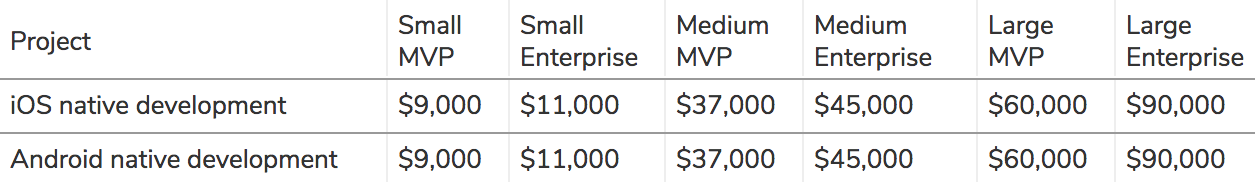
\includegraphics[width=0.95\textwidth]{img/nativeappkost.png}
	\caption{Kostprijs ontwikkeling native applicatie (\cite{NativeDevelopmentCost})}
	\label{fig:nativeappkost}
\end{figure}

Uit sectie \ref{sec:nativeversuscross} valt te besluiten dat er ook redenen zijn waarom bedrijven nu net wel native applicaties willen in plaats van cross-platform applicaties. 

Momenteel is er meer dan genoeg keuze om applicaties voor verschillende platformen tegelijkertijd te ontwikkelen. Met Kotlin/Native komt er een nieuw framework zich aanbieden. Dit framework is nog zeer jong en er bestaat bijna geen documentatie. Ontwikkelaars die dit framework willen gebruiken moeten momenteel zelf de werking van Kotlin/Native proberen achterhalen. Daarom is het belangrijk om te bestuderen of Kotlin een mogelijkheid biedt tot een nieuwe cross-platform programmeertaal, hoe de compiler van Kotlin ervoor kan zorgen dat het op meerdere platformen kan draaien en hoe men nu juist gebruik kan maken van Kotlin/Native. 

Voor Endare heeft deze bachelorproef een grote meerwaarde aangezien zij iedere dag met cross-platform frameworks aan de slag moeten. Kotlin/Native zou de mogelijkheid geven om native applicaties te ontwikkelen in combinatie met een domeinlogica die gedeeld wordt tussen de verschillende platformen.

%Uit je probleemstelling moet duidelijk zijn dat je onderzoek een meerwaarde heeft voor een concrete doelgroep. De doelgroep moet goed gedefinieerd en afgelijnd zijn. Doelgroepen als ``bedrijven,'' ``KMO's,'' systeembeheerders, enz.~zijn nog te vaag. Als je een lijstje kan maken van de personen/organisaties die een meerwaarde zullen vinden in deze bachelorproef (dit is eigenlijk je steekproefkader), dan is dat een indicatie dat de doelgroep goed gedefinieerd is. Dit kan een enkel bedrijf zijn of zelfs één persoon (je co-promotor/opdrachtgever).

\section{Onderzoeksvraag}
\label{sec:onderzoeksvraag}
De onderzoeksvragen voor deze bachelorproef zijn: 
\begin{itemize}
	\item Hoe zorgt de Kotlin compiler ervoor dat Kotlin op verschillende platformen kan gebruikt worden?
	\item Wat is de werking van Kotlin/Native?
	\item In hoeverre kan Kotlin gebruikt worden voor cross-platform applicatieontwikkeling?
\end{itemize}
%Wees zo concreet mogelijk bij het formuleren van je onderzoeksvraag. Een onderzoeksvraag is trouwens iets waar nog niemand op dit moment een antwoord heeft (voor zover je kan nagaan). Het opzoeken van bestaande informatie (bv. ``welke tools bestaan er voor deze toepassing?'') is dus geen onderzoeksvraag. Je kan de onderzoeksvraag verder specifiëren in deelvragen. Bv.~als je onderzoek gaat over performantiemetingen, dan 

\section{Onderzoeksdoelstelling}
\label{sec:onderzoeksdoelstelling}
Voor deze bachelorproef zijn er verschillende criteria van succes:
\begin{itemize}
	\item De werking van de compiler, die Kotlin gebruikt, documenteren
	\item Goede documentatie opstellen over de werking van Kotlin/Native
	\item Bepalen in hoeverre Kotlin gebruikt kan worden als cross-platform programmeertaal
\end{itemize}
%Wat is het beoogde resultaat van je bachelorproef? Wat zijn de criteria voor succes? Beschrijf die zo concreet mogelijk.

\section{Opzet van deze bachelorproef}
\label{sec:opzet-bachelorproef}
% Het is gebruikelijk aan het einde van de inleiding een overzicht te
% geven van de opbouw van de rest van de tekst. Deze sectie bevat al een aanzet
% die je kan aanvullen/aanpassen in functie van je eigen tekst.

De rest van deze bachelorproef is als volgt opgebouwd:

In Hoofdstuk~\ref{ch:stand-van-zaken} wordt een overzicht gegeven van de stand van zaken binnen het onderzoeksdomein, op basis van een literatuurstudie.

In Hoofdstuk~\ref{ch:methodologie} wordt de methodologie toegelicht en worden de gebruikte onderzoekstechnieken besproken om een antwoord te kunnen formuleren op de onderzoeksvragen.

In Hoofdstuk~\ref{ch:compiler} zal onderzocht worden, via een literatuurstudie, wat de werking is van de Kotlin compiler. Hoe ervoor kan gezorgd worden dat Kotlin ook op apparaten zonder een JVM kan draaien.

In Hoofdstuk~\ref{ch:kotlinnative} zal Kotlin/Native bestudeerd worden. Hierin zal de werking van Kotlin/Native gedocumenteerd worden.

In Hoofdstuk~\ref{ch:praktisch} zal er praktisch een Kotlin/Native project worden uitgewerkt.

In Hoofdstuk~\ref{ch:conclusie}, tenslotte, wordt de conclusie gegeven en een antwoord geformuleerd op de onderzoeksvragen. Daarbij wordt ook een aanzet gegeven voor toekomstig onderzoek binnen dit domein.


\chapter{Stand van zaken}
\label{ch:stand-van-zaken}

% Tip: Begin elk hoofdstuk met een paragraaf inleiding die beschrijft hoe
% dit hoofdstuk past binnen het geheel van de bachelorproef. Geef in het
% bijzonder aan wat de link is met het vorige en volgende hoofdstuk.

% Pas na deze inleidende paragraaf komt de eerste sectiehoofding.

Dit hoofdstuk bevat je literatuurstudie. De inhoud gaat verder op de inleiding, maar zal het onderwerp van de bachelorproef *diepgaand* uitspitten. De bedoeling is dat de lezer na lezing van dit hoofdstuk helemaal op de hoogte is van de huidige stand van zaken (state-of-the-art) in het onderzoeksdomein. Iemand die niet vertrouwd is met het onderwerp, weet er nu voldoende om de rest van het verhaal te kunnen volgen, zonder dat die er nog andere informatie moet over opzoeken \autocite{Pollefliet2011}.

Je verwijst bij elke bewering die je doet, vakterm die je introduceert, enz. naar je bronnen. In \LaTeX{} kan dat met het commando \texttt{$\backslash${textcite\{\}}} of \texttt{$\backslash${autocite\{\}}}. Als argument van het commando geef je de ``sleutel'' van een ``record'' in een bibliografische databank in het Bib\TeX{}-formaat (een tekstbestand). Als je expliciet naar de auteur verwijst in de zin, gebruik je \texttt{$\backslash${}textcite\{\}}.
Soms wil je de auteur niet expliciet vernoemen, dan gebruik je \texttt{$\backslash${}autocite\{\}}. In de volgende paragraaf een voorbeeld van elk.

\textcite{Knuth1998} schreef een van de standaardwerken over sorteer- en zoekalgoritmen. Experten zijn het erover eens dat cloud computing een interessante opportuniteit vormen, zowel voor gebruikers als voor dienstverleners op vlak van informatietechnologie~\autocite{Creeger2009}.

\lipsum[7-20]

%%=============================================================================
%% Methodologie
%%=============================================================================

\chapter{Methodologie}
\label{ch:methodologie}

%% TODO: Hoe ben je te werk gegaan? Verdeel je onderzoek in grote fasen, en
%% licht in elke fase toe welke stappen je gevolgd hebt. Verantwoord waarom je
%% op deze manier te werk gegaan bent. Je moet kunnen aantonen dat je de best
%% mogelijke manier toegepast hebt om een antwoord te vinden op de
%% onderzoeksvraag.

Vooraleer er aan de slag kon worden gegaan met het uittesten van Kotlin Native, of het analyseren van voorbeeldprojecten van JetBrains, was het belangrijk om te onderzoeken hoe het nu komt dat Kotlin Native op verschillende platformen kan draaien. Kotlin is oorspronkelijk, net zoals Java, een programmeertaal die gebruik maakt van de Java Virtual Machine. Het is daarom nuttig te onderzoeken hoe het mogelijk is gemaakt om Kotlin cross-platform te gebruiken. Dit is gebeurd aan de hand van een literatuurstudie. Het was niet nodig om dit praktisch te doen aangezien dit geen meerwaarde zou bieden aan deze bachelorproef. Kotlin/Native maakt gebruik van de LLVM compiler. Deze literatuurstudie is uitgevoerd aan de hand van de aosabook van LLVM, \textcite{aosa}, een zeer uitgebreide documentatie. 

Daarna werden de voorbeeldprojecten van JetBrains, geschreven in Kotlin/Native, geanalyseerd om de werking van dit framework te achterhalen. Hierbij was het de bedoeling om te onderzoeken hoe het mogelijk was, om in een zeer vroeg stadium van Kotlin/Native, reeds aan de slag te gaan met dit framework. Dit is begonnen met het downloaden van de code van de repositories van Kotlin/Native en de Kotlin multiplatform projects. Dit was niet gemakkelijk. Vaak waren er problemen met verkeerde versies of programma's die ontbraken op de computer. Na enige tijd kon er aan de slag worden gegaan met de projecten. In eerste instantie werden er dingen gewijzigd in het originele project van Kotlin/Native zelf om te kijken hoe alle modules, klassen, gradle bestanden werkten en gelinkt waren.

Eenmaal de werking van Kotlin Native duidelijk was, was het de bedoeling om zelf aan de slag te gaan met dit framework en een kleine cross-platform applicatie te schrijven. Hierbij werd er eerst een Kotlin/Native project opgezet, wat toch enige tijd in beslag heeft genomen. Eens het project was opgezet kon de applicatie gebouwd worden. Het prototype dat is gemaakt is een kleine shopping cart applicatie.



% Voeg hier je eigen hoofdstukken toe die de ``corpus'' van je bachelorproef
% vormen. De structuur en titels hangen af van je eigen onderzoek. Je kan bv.
% elke fase in je onderzoek in een apart hoofdstuk bespreken.

%%=============================================================================
%% Methodologie
%%=============================================================================

\chapter{De compilatie van Kotlin/Native}
\label{ch:compiler}
Kotlin is een programmeertaal die gebruik maakt van de JVM. Sinds de beslissing van JetBrains om zich ook te focussen op cross-platform development, moesten ze met een oplossing komen voor de JVM. De JVM wordt namelijk niet ondersteund op alle besturingssystemen. Zo ondersteunen bijvoorbeeld MacOS en iOS (mobile) geen JVM. JetBrains moest dus op zoek gaan naar een oplossing... de LLVM compiler. Deze literatuurstudie is uitgevoerd aan de hand van de aosabook van LLVM, \textcite{aosa}, een zeer uitgebreide documentatie. 

\section{Wat is LLVM?}
Het LLVM-project is een verzameling modulaire en herbruikbare compiler- en toolchaintechnologieën. Het project is ontwikkeld door de LLVM developer group, waarvan Vikram Adve en Chris Lattner de originele ontwikkelaars zijn. De naam 'LLVM' zelf is geen acroniem, het is de volledige naam van het project. Ondanks de naam heeft LLVM weinig te maken met de traditionele virtuele machines.

Het LLVM-project begon als een onderzoeksproject aan de universiteit van Illinois, met als doel een compilatiestrategie aan te bieden die in staat is om zowel statische als dynamische compilatie van programmeertalen aan te bieden. Een voorbeeld van een statische taal is Java, een voorbeeld van een dynamische taal is Javascript. Zowel beide types van programmeertalen kunnen dus gecompileerd worden door LLVM.

Sinds het ontstaan van LLVM is het project uitgegroeid tot een overkoepelend project dat bestaat uit een aantal deelprojecten. Veel van deze deelprojecten worden momenteel sterk gebruikt bij commerciële en open-source projecten en zelfs in academisch onderzoek.

Het grote voordeel van het gebruik van LLVM is de veelzijdigheid, flexibiliteit en herbruikbaarheid. Dit wil zeggen dat het zo goed als in ieder soort project kan worden geïntegreerd. Het wordt daarom tegenwoordig gebruikt voor een groot aantal verschillende taken, dit gaande van het compileren van enkele kleine code-projecten tot het compileren van code voor massieve computers.

\subsection{Deelprojecten LLVM}
Enkele voorbeelden van deelprojecten van de LLVM developers group:
\begin{itemize}
	\item \textbf{Clang} is een LLVM native C/C++/Objective-C compiler dat als doel heeft om verbazingwekkend snelle compilaties aan te bieden. Het zorgt overigens voor nuttige fout- en waarschuwingsberichten.
	\newline
	\item Het \textbf{LLDB} project bouwt verder op libraries die aangeboden worden door LLVM en Clang om te zorgen voor een native debugger.
	\newline
	\item Het \textbf{libc++} en \textbf{libc++ ABI} project voorziet een krachtige implementatie van de standaard C++ bibliotheek, met ondersteuning voor C++11. 
\end{itemize}

\section{De werking van LLVM}
LLVM is dus een bibliotheek die gebruikt wordt om tussenliggende en/of machine-code te genereren en optimaliseren. Maar wat is nu de exacte werking van deze compiler?

\subsection{De werking van een standaard compiler}
Het meest populaire ontwerp voor een statische compiler, zoals de meeste C-compilers, is het driefasenontwerp waarbij de belangrijkste componenten de \textbf{front-end}, de \textbf{optimizer} en de \textbf{back-end} zijn. 

\begin{figure} [ht]
	\centering
	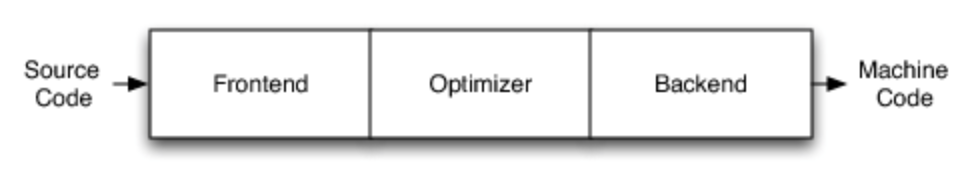
\includegraphics[width=0.95\textwidth]{img/driefasenmodel}
	\caption{Driefasenontwerp (\cite{aosa})}
	\label{fig:driefasenontwerp}
\end{figure}

\subsubsection{De front-end}
De front-end zorgt voor de analyse van de broncode. Deze heeft dus als taak om ervoor te zorgen dat geen code gecompileerd kan worden waarbij fouten aanwezig zijn. Dit gebeurt door het opstellen van een taalspecifieke abstracte syntaxboom om de syntaxcode voor te stellen. Deze syntaxboom wordt optioneel geconverteerd naar een nieuwe boom voor optimalisatie en de optimizer en de back-end worden uitgevoerd aan de hand van deze boom. De JVM is ook een implementatie van dit driefasenontwerp. Een voorbeeld van een syntaxboom is te zien in figuur \ref{fig:syntaxtree}.

\begin{figure} [ht]
	\centering
	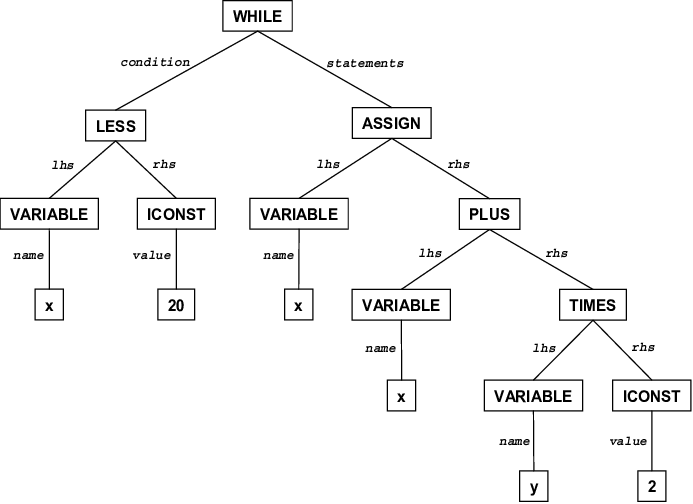
\includegraphics[width=0.95\textwidth]{img/syntaxtree.png}
	\caption{Taalspecifieke abstracte syntaxboom (\cite{ResearchGate})}
	\label{fig:syntaxtree}
\end{figure}

\subsubsection{De optimizer}
De optimizer is verantwoordelijk, zoals de naam het zelfs zegt, voor het uitvoeren van een breed gamma van transformaties om de uitvoeringstijd van de code te optimaliseren. Dit wordt gedaan door het elimineren van overtollige berekeningen, maar dit is meestal afhankelijk van de taal die gebruikt werd en de doelarchitectuur.

\subsubsection{De back-end}
De back-end, ook bekend als de codegenerator, gaat de code gaan mappen naar een instructieset. Naast het maken van deze instructieset is het ook verantwoordelijk om ervoor te zorgen dat deze instructieset gebruik maakt van de ongewone kenmerken van de ondersteunde architectuur. Iedere architectuur is namelijk anders en de instructieset moet dus met iedere architectuur kunnen werken. 

\subsection{Meerdere front- en backends}
Het grote voordeel van dit driefasenontwerp treedt op wanneer een compiler besluit om meerdere brontalen en architecturen te ondersteunen. Indien de optimizer een gemeenschappelijke code representatie gebruikt, dan kan een front-end geschreven worden voor elke taal die gecompileerd kan worden naar die gemeenschappelijke representatie, en een back-end kan worden geschreven voor elke doelarchitectuur dat daaruit kan compileren. Op figuur \ref{fig:llvmdriefasen} is te zien dat door de common optimizer te gebruiken, er meerdere front-ends kunnen worden geschreven en meerdere doelarchitecturen kunnen worden ondersteund.

Met dit ontwerp, indien men wenst een nieuwe brontaal te ondersteunen, moet men enkel een nieuwe front-end schrijven maar de bestaande optimizer en back-end kunnen worden hergebruikt. Indien deze delen (front-end, optimizer en back-end) niet waren gescheiden, zou het implementeren van een nieuwe brontaal vereisen om helemaal opnieuw te beginnen, dus een volledig nieuwe compiler te schrijven. Indien men N doelarchitecturen heeft en M brontalen, dan zou men N*M compilers hebben.

Nog een voordeel van dit ontwerp is dat deze soorten van compilers een veel bredere set van programmeurs kan tevreden stellen. Dit is minder het geval indien men slechts één brontaal en doelarchitectuur zou ondersteunen. 

\begin{figure} [ht]
	\centering
	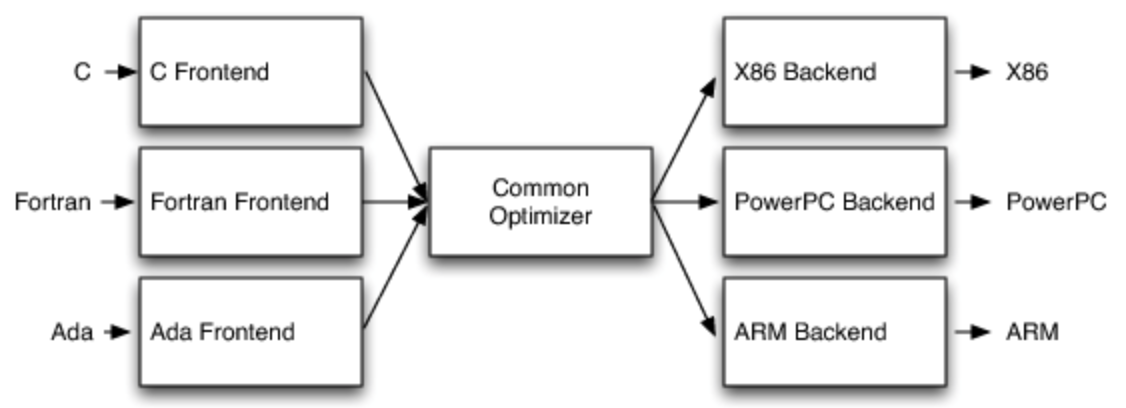
\includegraphics[width=0.95\textwidth]{img/llvmdriefasen}
	\caption{Meerdere front- en backends (\cite{aosa})}
	\label{fig:llvmdriefasen}
\end{figure}

\section{Verschil met LLVM}
\label{sec:difference-llvm}
In een LLVM-gebaseerde compiler heeft de front-end dezelfde taak als de front-end in een normale compiler. De code wordt daarna door de front-end vertaald naar LLVM intermediate representation (IR), dit meestal door het opbouwen van een syntaxboom en deze later te converteren naar IR. De IR is eigenlijk het hart van de LLVM. Het is een low-level programmeertaal die zeer dicht aansluit bij assembly code. Deze IR heeft als taak om de code te verbeteren, waarna deze code in een soort van codegenerator wordt gestoken waarbij deze wordt omgezet naar native machinecode. 

In een korte notendop: de front-end krijgt een brontaal binnen en gaat deze taal parsen, valideren en analyseren. Hij stelt de syntaxboom op en zet deze om naar LLVM IR. De optimizer gaat de code optimaliseren en stuurt de IR code naar de back-end die dient als codegenerator met als resultaat machinecode.

\begin{figure} [ht]
	\centering
	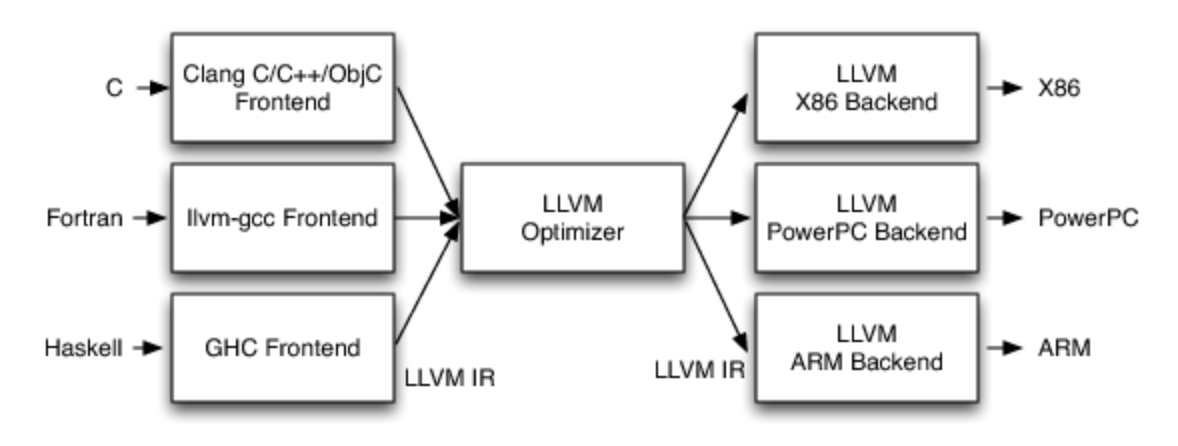
\includegraphics[width=0.95\textwidth]{img/llvmirdriefasen}
	\caption{LLVM implementatie van driefasenontwerp (\cite{aosa})}
	\label{fig:llvmirdriefasen}
\end{figure}

\section{LLVM en Kotlin}
Kotlin/Native is een technologie dat Kotlin via LLVM direct compileert naar machine code. De Kotlin/Native compiler produceert zelfstandige uitvoerbare bestanden die zonder virtuele machine kunnen worden uitgevoerd. Hierdoor is het mogelijk om Kotlin te gebruiken op ieder platform of besturingssysteem.

\section{Java Virtual Machine (JVM)}
\label{sec:jvm}
De Java Virtual Machine, ook wel JVM genoemd, is een virtuele machine voor het uitvoeren van Java bytecode \autocite{TechopediaBytecode}. Deze bytecode is een object-georiënteerde code die gecompileerd is om op een virtuele machine te worden uitgevoerd. De code kan op elk besturingssysteem of platform, waarvoor er een JVM beschikbaar is, worden gebruikt. De virtuele machine transformeert de code, geschreven in een bepaalde programmeertaal, in machinetaal die door de CPU\footnote{Central Processing Unit} van een systeem kan worden uitgevoerd, aangezien platformen andere interpretatietechnieken kunnen gebruiken. Bij de JVM zal de bytecode meestal het resultaat zijn van de compilatie van Java-code. Echter kunnen talen zoals Scala, Clojure en Groovy ook uitgevoerd worden op deze virtuele machine. De JVM heeft kennis van geheugenbeheer, optimalisatie van de uitvoering van de applicatie en garbage collection. Daarnaast begrijpt de JVM het concept van objecten en virtuele methode aanroepen. De gebruiker hoeft hierdoor geen rekening te houden met deze drie zaken \autocite{TechopediaJVM}. 

\section{LLVM en JVM}
LLVM en JVM zijn twee aparte dingen. De JVM is, zoals te lezen in sectie \ref{sec:jvm}, een vertaler die broncode omzet naar machinetaal die door de processor van een computer onmiddelijk kan worden uitgevoerd. Het is een high-level virtuele machine aangezien deze kennis heeft van zaken zoals de garbage collection, geheugenbeheer en objecten.

De LLVM is een low-level register gebaseerde compilatie technologie. Het neemt de LLVM IR, zie sectie \ref{sec:difference-llvm}, en gaat deze overbrengen naar native uitvoerbare bestanden voor een specifiek platform. LLVM kan tijdens het vertaalproces naar IR veel optimalisaties uitvoeren.

%De LLVM is een low-level register gebaseerde compilatie technologie. Het is ontworpen om onderliggende hardware te abstraheren en een lijn te trekken tussen de front-end en de back-end van een compileerprogramma.

%De JVM is een high-level stack gebaseerde virtuele machine. De JVM biedt garbage collection aan, heeft kennis van objecten en virtuele methode aanroepen. JVM biedt dus een veel hogere infrastructuur voor taalinteroperabiliteit.

%Het grote verschil tussen LLVM en JVM is dus het niveau waarop beide werken.

%%=============================================================================
%% Methodologie
%%=============================================================================

\chapter{De werking van Kotlin/Native}
JetBrains heeft met Kotlin/Native de interesse van elke cross-platform ontwikkelaar getrokken. Niemand had verwacht dat Kotlin uitgebreid ging worden met een cross-platform framework. Zo zal JetBrains met Kotlin/Native een nieuwe markt betreden, het maken van native applicaties in combinatie met het delen van domeinlogica tussen de verschillende ondersteunde platformen.
\label{ch:kotlinnative}

\section{Wat is Kotlin/Native?}
Kotlin/Native is een technologie die zorgt voor de compilatie van Kotlin naar native binaire bestanden die zonder VM draaien. Kotlin/Native maakt gebruikt van een LLVM gebasseerde backend voor de Kotlin-compiler en een native implementatie van de Kotlin bibliotheek. Origineel werd Kotlin/Native uitgevonden om compilatie van Kotlin mogelijk te maken op platformen die geen virtuele machines, zoals de JVM, ondersteunen. Een voorbeeld hiervan is iOS dat geen ondersteuning biedt voor de JVM.

\iffalse
%TODO: Vragen
Kotlin Native ondersteunt volledig de interoperabiliteit met native code. Wat betreft het gebruik van Kotlin libraries, deze zijn volledig ter beschikking van de ontwikkelaar. Indien een bepaalde bibliotheek niet ondersteund wordt, bestaat er een tool om een tussenliggende bibliotheek te genereren van een C-header bestand, waardoor deze bibliotheek toch gebruikt kan worden.  Op macOS en iOS wordt samenwerking met Objective/C-code ook ondersteund.
\fi

Kotlin Native is momenteel heel jong en zit nog in volledige ontwikkeling. De eerste versie van Kotlin/Native werd vrijgegeven op 31 maart 2017. Er zijn reeds enkele versies aanwezig op de GitHub van JetBrains waar ontwikkelaars met aan de slag kunnen. De ondersteuning voor de IDE's is beschikbaar als een plugin voor CLion.

\section{Het delen van code in Kotlin/Native}
\label{sec:sharingcode}
Het doel van Kotlin/Native is om een framework aan te bieden dat gebruikt kan worden voor cross-platform ontwikkeling. De focus ligt niet op het maken van user interfaces, met alle functionaliteiten inbegrepen, via één codebase, maar wel op het delen van de domeinlogica. JetBrains wil dus via Kotlin/Native de mogelijkheid aanreiken om alle domeinlogica in een applicatie te hergebruiken op verschillende platformen en per platform de user interface op te bouwen.

Voordelen:
\begin{itemize}
	\item Hergebruik van de domeinlogica.
	\item Mogelijkheid om per platform, in de user interface, andere accenten naar voor te brengen.
\end{itemize}

Nadelen:
\begin{itemize}
	\item Verplichting om meerdere user interfaces op te bouwen (indien men meerdere platformen wil ondersteunen).
	\item Grotere kosten en meer tijd nodig om beide applicaties te ontwikkelen (Android en iOS).
	\item Opzet van dit soort projecten is (momenteel) niet gemakkelijk voor de onervaren gebruiker.
\end{itemize}

Figuur \ref{fig:sharingcode} toont hoe Kotlin/Native domeinlogica deelt over de verschillende platformen heen. Er wordt gebruik gemaakt van een \textbf{common} module. In deze module bevindt zich de gemeenschappelijke code, die gedeeld wordt met alle platformen en dus voor elk platform hetzelfde zal zijn. Daarnaast is er per platform dat ondersteund moet worden een aparte platformmodule. Deze platformmodules maken gebruik van de common module en er kan in deze platformmodules platformspecifieke code geschreven worden. De mogelijkheid is dus aanwezig om voor een bepaalde klasse, per platform een andere implementatie te voorzien. Zie sectie \ref{sec:expectandactual} voor een meer technische uitleg.

\begin{figure} [ht]
	\centering
	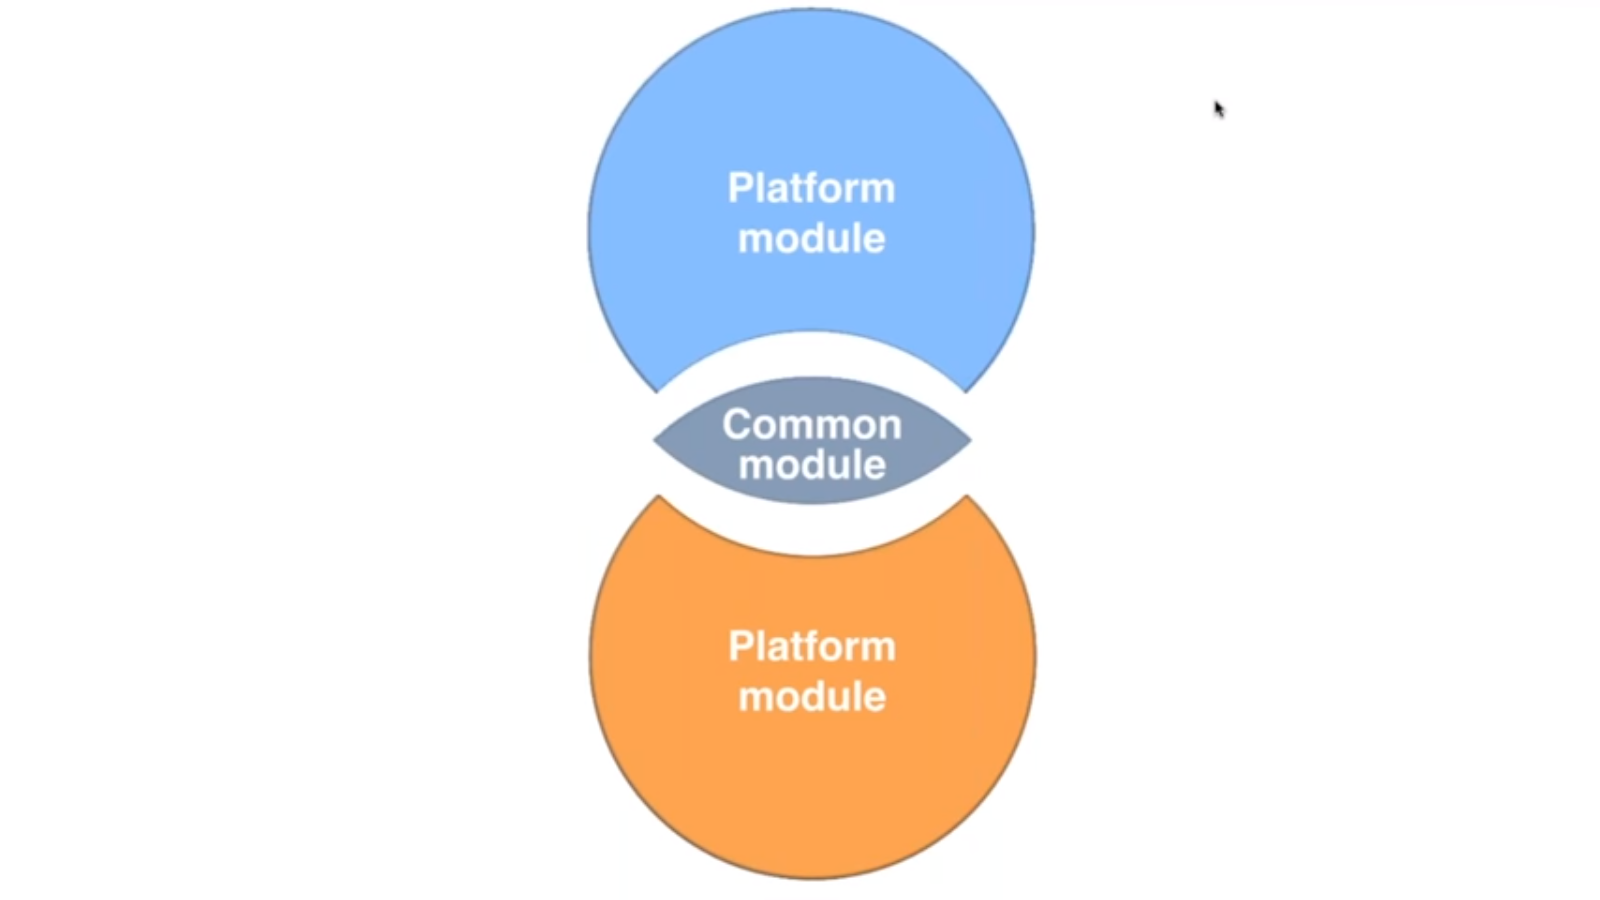
\includegraphics[width=0.95\textwidth]{img/sharingcode}
	\caption{Het delen van code in Kotlin Native (\cite{Developine})}
	\label{fig:sharingcode}
\end{figure}

\section{De structuur van een Kotlin/Native project}
\label{sec:knstructure}
Alvorens te beginnen met het ontwikkelen van een Kotlin/Native project is het belangrijk om na te gaan wat de structuur is waar een Kotlin/Native project moet aan voldoen. Er is namelijk geen IDE of plugin die een Kotlin/Native project volledig automatisch genereert, daarom is het essentieel dat er vanaf het begin een goede mappenstructuur wordt opgebouwd. Figuur \ref{fig:knstructuur} toont een goede structuur van een Kotlin/Native project.

\begin{figure} [ht]
	\centering
	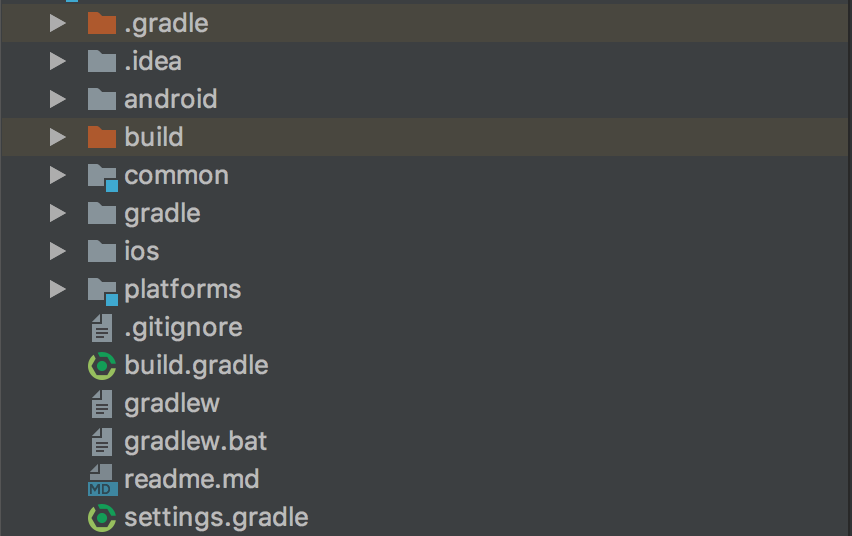
\includegraphics[width=0.95\textwidth]{img/kn-project-structure}
	\caption{Kotlin/Native structuur}
	\label{fig:knstructuur}
\end{figure}

Op deze figuur zijn dus een aantal mappen te vinden:
\begin{itemize}
	\item De \textbf{.gradle} map, automatisch gegenereerd, houdt alle instellingen en andere bestanden bij die gebruikt worden door Gradle om het project te bouwen. Dit wordt automatisch gegenereerd wanneer er een Gradle run wordt uitgevoerd.
	\item Voor dit voorbeeld werd IntelliJ gebruikt als IDE. IntelliJ zal de map, \textbf{.idea}, automatisch genereren om verschillende instellingen van het project bij te houden. Alle projectspecifieke instellingen zijn aanwezig in deze map.
	\item \textbf{android} bevat het volledige Android project.
	\item De \textbf{build} map bevat informatie over de laatste uitgevoerd build.
	\item De \textbf{common} map bevat gemeenschappelijke code dat over de verschillende platformen wordt gedeeld.
	\item De \textbf{gradle} map, automatisch gegenereerd, bevat een properties bestand. In dit bestand worden enkele belangrijke properties onthouden, zoals de locatie van de gradle installatie.
	\item \textbf{ios} bevat het volledige iOS project.
	\item De \textbf{platforms} map bevat voor ieder platform, dat men wenst te ondersteunen, een map. In dit voorbeeld zijn er dus twee mappen, een iOS en Android map. De bedoeling is om hierin specifieke code te schrijven die varieert per platform. Zie sectie \ref{sec:sharingcode} voor meer informatie.
\end{itemize}

\section {Expect en actual klassen}
\label{sec:expectandactual}
Stel dat men wenst om een ABCMethods Kotlin klasse te hebben die de methodes callA(), callB() en callC() heeft, maar waarvan de implementatie verschillend is per platform.

In de common module wordt de ABCMethods klasse aangemaakt. Hierbij wordt het keyword \textit{expect} gebruikt. Het keyword zegt bijna zelf waarvoor het gebruikt moet worden: er wordt een ABCMethods klasse 'verwacht' voor ieder platform. Het expect keyword kan ook vergeleken worden met een standaard Java interface.

\begin{lstlisting}
expect class ABCMethods() {
	fun callA():String
	fun callB():String
	fun callC():String
}
\end{lstlisting}

Met het \textbf{actual} keyword geven we aan dat deze klasse een concrete implementatie is van ABCMethods. De compiler zal in eerste instantie zoeken naar de ABCMethods klasse in de common module. Hij zal daar merken dat ABCMethods een expect klasse is waardoor hij naar de platformspecifieke folder zal gaan en daar de actual klasse van ABCMethods zal gebruiken. Voor ieder platform wordt dus een concrete implementatie voorzien van de ABCMethods klasse.

Een mogelijke implementatie voor iOS:
\begin{lstlisting}
actual class ABCMethods actual constructor() {
	actual fun callA():String {
		return "Calling A from iOS"
	}
	
	actual fun callB():String {
		return "Calling B from iOS"
	}
	
	actual fun callC():String {
		return "Calling C from iOS"
	}
}
\end{lstlisting}

Een mogelijke implementatie voor Android:
\begin{lstlisting}
actual class ABCMethods actual constructor() {
	actual fun callA():String {
		return "Calling A from Android"
	}
	
	actual fun callB():String {
		return "Calling B from Android"
	}
	
	actual fun callC():String {
		return "Calling C from Android"
	}
}
\end{lstlisting}

Door gebruik te maken van Kotlin/Native is het niet nodig om zelf aan te geven welk bestand de compiler moet gebruiken voor welk platform. De compiler zal detecteren welk platform er gebruikt wordt en het juiste bestand gebruiken.

\section{Gemeenschappelijke klassen}
Naast de expect en actual klassen, die ervoor zorgen dat we platformspecifieke code kunnen schrijven en dus een onderscheid kunnen maken tussen de verschillende ondersteunde platformen, kunnen we ook klassen voorzien die voor alle platformen hetzelfde zijn. De implementatie van deze klasse is voor ieder platform hetzelfde.

\begin{lstlisting}
class Example {
	private var name: String
	
	constructor() {
		this.name = "Ilias.vw"
	}
	
	fun helloKotlin(): String {
		return "Hello Kotlin Native, from $name"
	}
}
\end{lstlisting}

\section {Het gebruiken van de Kotlin code}
\label{sec:use-ios-code}
Maar hoe kan de gemeenschappelijke en platformspecifieke code gebruikt worden? Simpel. Bij een Android project kunnen we de Kotlin code gebruiken door simpelweg de bibliotheek te importeren. Dit is niks meer dan een import bovenaan in de Android activity. iOS gerelateerde code zal gedeeld worden via een iOS framework dat gegenereerd wordt door Kotlin/Native. Dit framework zal toegevoegd worden in de build phases van het xcode project. Zie sectie \ref{sec:ios-stap6} voor meer informatie.
\chapter{Praktische uitwerking Kotlin/Native}
\label{ch:praktisch}
In dit hoofdstuk zal er praktisch een Kotlin/Native project worden opgebouwd. De bedoeling is om aan de hand van een voorbeeld de volledige werking uit te leggen. In dit voorbeeld zal er een simpele applicatie gebouwd worden, gericht op Android en iOS, waarbij gebruikers een shopping cart kunnen aanmaken, producten kunnen bekijken en toevoegen aan de shopping cart en kunnen bekijken welke producten reeds in hun winkelmandje aanwezig zijn. Het volledige project is te vinden op https://github.com/Iliasvw/kotlin-native-example.

\section{Domeinmodel}
Aangezien het doel van Kotlin/Native het delen van business logica is, is het handig om op voorhand na te denken over het domeinmodel. Welke klassen heb ik nodig, welke attributen en methodes moeten deze klassen hebben, is er eventueel een verschil in klassen tussen Android en iOS? Een domeinmodel geeft je ook een duidelijk overzicht over je applicatie. Zie figuur \ref{fig:domeinmodel-kn} om het domeinmodel te zien van deze voorbeeldapplicatie.

\begin{figure} [ht]
	\centering
	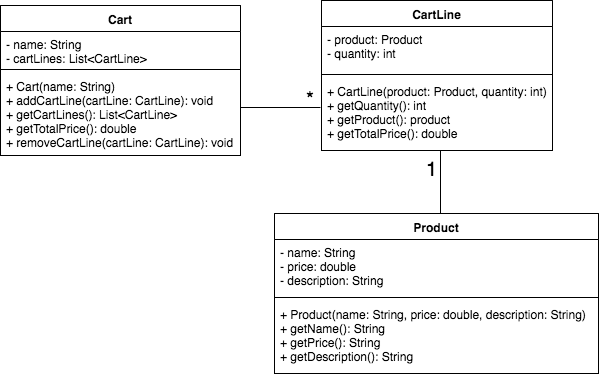
\includegraphics[width=0.95\textwidth]{img/domeinmodel.png}
	\caption{Klassendiagram domeinlogica}
	\label{fig:domeinmodel-kn}
\end{figure}

\section{Requirements}
Om gebruik te kunnen maken van Kotlin/Native voor het ontwikkelen van cross-platform applicaties (iOS \& Android), zijn er enkele vereisten:
\begin{itemize}
	\item \textbf{Android studio} voor het ontwikkelen van de Android applicatie.
	\item \textbf{Xcode} voor het ontwikkelen van de iOS applicatie (toestel met MacOS is vereist).
	\item \textbf{IntelliJ IDEA} (optioneel) voor het opzetten van het project. Dit kan eventueel met een andere IDEA, die gradle projecten ondersteunt, worden opgezet.
	\item \textbf{Gradle} om gebruik te kunnen maken van de Kotlin/Native compiler en plugin. Deze wordt geïnstalleerd bij het instellen van IntelliJ IDEA of Android Studio.
\end{itemize}

\section{Stap 1: project initiatie}
De eerste stap in het ontwikkelen van een Kotlin/Native project is het maken van een nieuwe map op een gewenste locatie op de harde schijf van je computer. Hierin zal er een eerste bestand worden aangemaakt: \textbf{build.gradle}.

\begin{lstlisting}
subprojects {
 buildscript {
  ext.kotlin_version = '1.2.31'
  ext.kotlin_native_version = '0.6.2'
		
  repositories {
   jcenter()
   google()
   maven { url "http://kotlin.bintray.com/kotlinx" }
   maven { url "https://plugins.gradle.org/m2/" }
   maven { url "https://dl.bintray.com/jetbrains/ kotlin-native-dependencies" }
  }

  dependencies {
   classpath "org.jetbrains.kotlin:kotlin-gradle-plugin: $kotlin_version"
   classpath 'com.android.tools.build:gradle:3.0.1'
   classpath "org.jetbrains.kotlin:kotlin-native-gradle-plugin: $kotlin_native_version"
  }
 }
	
 group 'ilias.vw'
 version '1.0-SNAPSHOT'
	
 repositories {
  jcenter()
  maven { url "http://kotlin.bintray.com/kotlinx" }
 }
	
 tasks.withType(Test) {
  testLogging {
   showStandardStreams = true
   events "passed", "failed"
  }
 }
}
\end{lstlisting}
\subsection{Versies}
Bovenaan geven we aan welke versie van Kotlin en Kotlin/Native we willen gebruiken. Dit zijn beide de nieuwste versies. Opgelet, het is niet altijd vanzelfsprekend om de laatste versie van Kotlin/Native te gebruiken. Er wordt voortdurend gewerkt aan Kotlin/Native en nieuwe dingen worden continu gepushed op de Github repository. Het kan al eens gebeuren dat sommige features niet altijd even goed werken, wat voor problemen kan zorgen bij de ontwikkeling van de applicatie. Bij twijfels, neem een minder recente versie van de Kotlin/Native plugin.

\subsection{Repositories}
In de repositories tag worden de juiste repositories gelinkt:
\begin{itemize}
	\item \textbf{Kotlinx} bevat alle coroutines\footnote{Programmaonderdelen die asynchroon programmeren vergemakkelijken door gecompliceerde logica in bibliotheken te steken} die Kotlin kan gebruiken.
	\item \textbf{Gradle}
	\item \textbf{Kotlin-native-dependencies} stelt alle dependencies, die Kotlin/Native nodig heeft, ter beschikking.
\end{itemize}

\subsection{Dependencies}
In de dependencies tag worden de juiste dependencies gelinkt:
\begin{itemize}
	\item \textbf{Kotlin-gradle} laadt de Kotlin-gradle plugin met de versie van Kotlin die wordt aangegeven bovenaan het build script. Deze plugin zorgt voor het compileren van Kotlin bronnen en modules.
	\item \textbf{Android build tools} is nodig voor het bouwen van de Android applicatie.
	\item \textbf{Kotlin-native-gradle-plugin} is de Kotlin/Native plugin die gebruikt zal worden om te zorgen voor een cross-platform applicatie.
\end{itemize}

\subsection{Overige informatie}
\label{sec:overige}
\begin{itemize}
	\item \textbf{Group} stelt het groupId van het project in.
	\item \textbf{Version} geeft de versie van het project weer.
	\item \textbf{testLogging} wordt gebruikt voor het uitvoeren van de testen.
\end{itemize}

\section{Stap 2: project structuur}
Nadat het build.gradle bestand gemaakt is, is het de bedoeling om via IntelliJ IDEA het gradle bestand te importeren. Zie figuur \ref{fig:stap2-import}. IntelliJ zal een dialoogvenster openen, waarbij het build.gradle bestand moet worden geopend. De IDE zal hierna het build.gradle bestand uitvoeren en het genereert enkele bestanden.

\begin{figure} [ht]
	\centering
	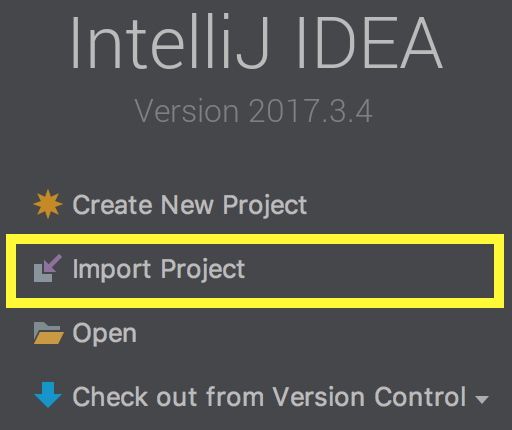
\includegraphics[width=0.60\textwidth]{img/stap2-import.png}
	\caption{Importeren van een project}
	\label{fig:stap2-import}
\end{figure}

In de huidige versie van Kotlin/Native worden de overige mappen nog niet automatisch aangemaakt. Alle andere mappen, die te zien zijn in figuur \ref{fig:knstructuur} moeten handmatig aangemaakt worden. Deze mappenstructuur zal geleidelijk aan opgebouwd worden naargelang de stappen vorderen.

\section{Stap 3: Common map }
In de common map wordt alle gemeenschappelijke code geschreven. In deze map moet er aan een bepaalde structuur worden voldaan, zie figuur \ref{fig:stap3-common}.

\begin{figure} [ht]
	\centering
	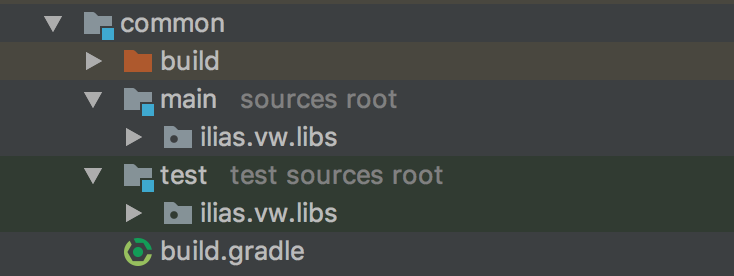
\includegraphics[width=0.60\textwidth]{img/stap3-common.png}
	\caption{Common module structuur}
	\label{fig:stap3-common}
\end{figure}

\subsection{Build map}
De build map bevat alle gecompileerde bestanden die genereerd worden door Kotlin/Native en worden bij iedere gradle run en/of build aangemaakt.

\subsection{Main en test map}
\label{sec:maintestcommon}
Zoals te zien is op figuur \ref{fig:stap3-common} heeft zowel de main als test map enkele subpackages. Deze beginnen met het groupId dat ingesteld is in sectie \ref{sec:overige} met daarin nog eens een 'libs' map. De naam van deze 'libs' map is vrij te kiezen, maar in dit voorbeeld wordt altijd 'libs' gebruikt.

De main map zal alle gemeenschappelijke klassen bevatten (expect en gewone klassen, zie sectie \ref{sec:expectandactual}).

De test map zal alle gemeenschappelijke test klassen bevatten, gebruikmakend van de klassen in de main map.

\subsection{Build.gradle}
Natuurlijk moet de common module ook gecompileerd worden door Kotlin/Native. Hiervoor is er een build.gradle nodig.

\begin{lstlisting}
apply plugin: 'kotlin-platform-common'

sourceSets {
 main.kotlin.srcDirs += 'main/'
 test.kotlin.srcDirs += 'test/'
}

dependencies {
 compile "org.jetbrains.kotlin:kotlin-stdlib-common:$kotlin_version"
 testCompile "org.jetbrains.kotlin:kotlin-test-annotations-common: $kotlin_version"
 testCompile "org.jetbrains.kotlin:kotlin-test-common:$kotlin_version"
}
\end{lstlisting}
De bovenste regel in de build.gradle geeft aan dat we gebruik maken van de kotlin-platform-common plugin. Deze zal verantwoordelijk zijn voor het compileren en delen van alle gemeenschappelijke code over de verschillende platformen.

Er worden ook twee sourceSets toegevoegd. SourceSets vertegenwoordigen een logische groep van Java/Kotlin bronnen.

Tenslotte worden er drie dependencies toegevoegd. De stdlib is verantwoordelijk verlenen van toegang tot de standaard bibliotheek van Kotlin. Hierdoor hebben we toegang tot collections, streams, annotations, ... Er worden nog twee test dependencies toegevoegd, één verantwoordelijk voor de annotations, de andere voor het opstellen en uitvoeren van de testen, zie sectie \ref{sec:testing} voor meer informatie over testen.

\section{Common code}
Uitwerking van de common code van de voorbeeldapplicatie.
\subsection{Cart}
\begin{lstlisting}
package ilias.vw.libs
	
class Cart constructor(name: String) {
 var name: String = name
 private var cartLines: List<CartLine> = mutableListOf()
	
 fun getCartLines(): List<CartLine> {
  return this.cartLines
 }
	
 fun addCartLine(cartLine: CartLine) {
  for (item in cartLines) {
   if (item.getProduct().getName() == cartLine.getProduct().getName()) {
    item.add(cartLine.getQuantity())
    return
   }
  }
  this.cartLines += cartLine
 }
	
 fun getTotalPrice(): Double {
  var totalPrice = 0.0
	
  for (line in cartLines) {
   totalPrice += line.getTotalPrice()
  }
	
  return totalPrice
 }
	
 fun removeCartLine(cartLine: CartLine) {
  this.cartLines -= cartLine
 }
}
\end{lstlisting}

\subsection{CartLine}
\begin{lstlisting}
package ilias.vw.libs

class CartLine {
 private val product: Product
 private val quantity: Int

 constructor(product: Product, quantity: Int) {
  this.product = product
  this.quantity = quantity
 }

 fun getProduct(): Product {
  return this.product
 }

 fun getQuantity(): Int {
  return this.quantity
 }

 fun getTotalPrice(): Double {
  return product.getPrice() * quantity
 }
}
\end{lstlisting}

\subsection{Product}
De product klasse is een expect klasse. Dit wil zeggen dat we voor iedere platform een andere implementatie hebben van deze klasse. Maar voor iedere platform verwachten we wel dat deze de getName, getPrice en getDescription methodes heeft.

\begin{lstlisting}
package ilias.vw.libs

expect class {
 fun getName(): String
 fun getPrice(): Double
 fun getDescription(): String
}
\end{lstlisting}

\section{Stap 4: platforms folder}
De platform folder bevat enkele subfolders, één subfolder per platform waarvoor men wenst te ontwikkelen. Bij dit voorbeeld zijn er dus twee subfolders aanwezig, namelijk Android en iOS. Zie figuur \ref{fig:stap4-structuur}. Per submap, hebben we opnieuw twee submappen, namelijk main en test. Net zoals bij de common map. 

\begin{figure} [ht]
	\centering
	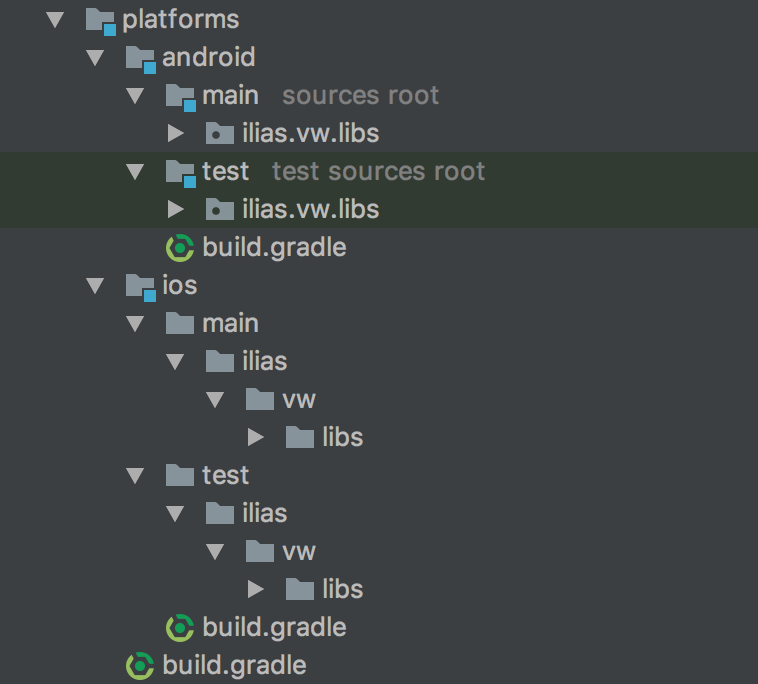
\includegraphics[width=0.60\textwidth]{img/stap4-structuur.png}
	\caption{Platforms module structuur}
	\label{fig:stap4-structuur}
\end{figure}

Zowel de main en test bevatten elk nog een map. Bij Android is dit een package die begint met het groupId, zie sectie \ref{sec:overige}, en eindigt met een willekeurige naam. In dit voorbeeld is dit opnieuw 'libs'. Dit dient identiek te zijn met de naam van de package gekozen in de common map, zie sectie \ref{sec:maintestcommon}. In het geval van iOS zijn dit geen packages maar eerder een mappenstructuur.

\subsection{android map}
\subsubsection{Build.gradle}
\begin{lstlisting}
apply plugin: 'kotlin-platform-jvm'

repositories {
 jcenter()
 maven { url "http://kotlin.bintray.com/kotlinx" }
}

sourceSets {
 main.kotlin.srcDirs += 'main/'
 test.kotlin.srcDirs += 'test/'
}

dependencies {
 compile "org.jetbrains.kotlin:kotlin-stdlib:$kotlin_version"
 expectedBy project(":common")

 testCompile "junit:junit:4.12"
 testCompile "org.jetbrains.kotlin:kotlin-test-junit: $kotlin_version"
 testCompile "org.jetbrains.kotlin:kotlin-test:$kotlin_version"
}
\end{lstlisting}

In deze build.gradle wordt er gebruik gemaakt van de kotlin-platform-jvm plugin. Android applicaties maken nog steeds gebruik van de JVM en dus ook deze android applicatie. 

De sourceSets worden ingesteld. Kotlin/Native zal steeds zoeken naar code in de map src/kotlin/main of src/kotlin/test, maar hier geven we aan dat code te vinden is in de main en test map en dus niet onder een src/kotlin/ map.

Tenslotte worden alle dependencies geladen en wordt er aangegeven dat de common module verwacht wordt die code bevat.

\subsubsection{Platformspecifieke code}
De platformspecifieke code voor Android. Graag willen we het product ook van een afbeelding voorzien en aangezien drawables in Android gemapt worden naar een Integerwaarde, wordt er een getal ingevuld in de constructor. De naam van het product wordt teruggeven met prefix 'Android'.
\begin{lstlisting}
package ilias.vw.libs

import java.io.Serializable

actual class Product: Serializable {
 private val name: String
 private val price: Double
 private val description: String
 private val productImage: Int

 actual constructor(name: String, price: Double, 
		description: String, productImage: Int) {
  this.name = name;
  this.price = price
  this.description = description
  this.productImage = productImage
 }

 actual fun getName(): String {
  return "Android: $name"
 }

 actual fun getPrice(): Double {
  return this.price
 }

 actual fun getDescription(): String {
  return this.description
 }

 actual fun getProductImage(): Int {
  return this.productImage
 }
}
\end{lstlisting}

\subsection{ios map}
\subsubsection{Build.gradle}
\label{sec:ios-build-gradle}
\begin{lstlisting}
apply plugin: 'konan'

konanArtifacts {
 framework('SharediOS', targets: ['iphone', 'iphone_sim']){
  enableDebug true
  enableMultiplatform true

  srcDir 'main'
 }

 library('test-library') {
  enableMultiplatform true
  srcDir 'main'
 }

 program('shared-ios-test') {
  srcDir 'test'
  commonSourceSet 'test'
  extraOpts '-tr'
  libraries {
   artifact 'test-library'
  }
 }
}

dependencies {
 expectedBy project(':common')
}
\end{lstlisting}

Zoals reeds te lezen is in sectie \ref{sec:use-ios-code} zal Kotlin/Native alle Kotlin code compileren naar een iOS framework. In de build.gradle wordt de naam van het framework en de toestellen (iPhone en iPhone simulators) dat men wenst te ondersteunen ingesteld.

De main map wordt als source directory ingesteld. Om ervoor te zorgen dat op iOS ook de testen kunnen worden uitgevoerd, wordt de main map ingesteld als bron voor alle testen, de test map wordt ingesteld als bron waar alle testen zijn gelokaliseerd.

Tenslotte wordt er opnieuw aangegeven dat we een common module verwachten die code bevat.

\subsubsection{Platformspecifieke code}
De platformspecifieke code voor iOS. In iOS heb je de mogelijkheid om afbeeldingen in te laten aan de hand van de naam van de imageset. Daardoor heeft de constructor een productImage die van het type String is. De naam van het product wordt teruggegeven met prefix 'iOS'.
\begin{lstlisting}
package ilias.vw.libs

actual class Product {
 private val name: String
 private val price: Double
 private val description: String
 private val productImage: String

 actual constructor(name: String, price: Double, 
		description: String, productImage: String) {
  this.name = name;
  this.price = price
  this.description = description
  this.productImage = productImage
 }

 actual fun getName(): String {
  return "iOS: $name"
 }

 actual fun getPrice(): Double {
  return this.price
 }

 actual fun getDescription(): String {
  return this.description
 }

 fun getProductImage(): String {
  return this.productImage
 }
}
\end{lstlisting}

\section{Stap 5: Android map}
In de android map is het de bedoeling om via Android Studio een nieuw project aan te maken. Bij het aanmaken van het project in Android Studio kan je de locatie van het project opgeven. Deze locatie moet zodanig ingesteld zijn dat het Android project een submap is van het Kotlin/Native project en waardoor het geïntegreerd zal worden in dit project.

\subsection{settings.gradle}
Voor we gebruik kunnen maken van de Kotlin klassen, moeten er eerst nog enkele wijzigingen gebeuren in de settings.gradle. De settings.gradle wordt vervangen door onderstaande code:

\begin{lstlisting}
include ':app'

include ':common'
project(":common").projectDir = new File("../common")

include ':platforms-android'
project(":platforms-android").projectDir = new File("../platforms/android")
\end{lstlisting}

Via de settings.gradle wordt er aangegeven om de common en platforms-android modules te includen in het project.

\subsection{build.gradle}
Tenslotte moet er nog een kleine wijziging doorgevoerd worden in de build.gradle van de app map. In de dependencies tag moet er enkele en alleen volgende lijn toegevoegd worden in de dependencies tag:

\begin{lstlisting}
implementation project(':platforms-android')
\end{lstlisting}

Hiermee wordt er aangegeven dat de android-specifieke implementatie te vinden is in platforms-android, waarvan de locatie is opgegeven in de settings.gradle. 

\section{Stap 6: iOS map}
\label{sec:ios-stap6}
Net zoals bij de android map, is het de bedoeling om via Xcode een nieuw Xcode project aan te maken dat ook een submap is van het Kotlin/Native project. Men kan zowel kiezen voor een Objective-C als Swift project aangezien het gecompileerde iOS framework zowel in beide projecten kan gebruikt worden.

\subsection{Gebruiken van het SharediOS framework}
Vooraleer men in Xcode kan gebruik maken van het SharediOS framework, moeten er een aantal dingen aangepast worden in de build phases van het project. Uit figuur \ref{fig:stap6-phases} kan worden afgeleid dat de build phases zijn aangepast. Volgende build phase moet worden toegevoegd: Compile Kotlin Native to iOS framework.
\begin{figure} [ht]
	\centering
	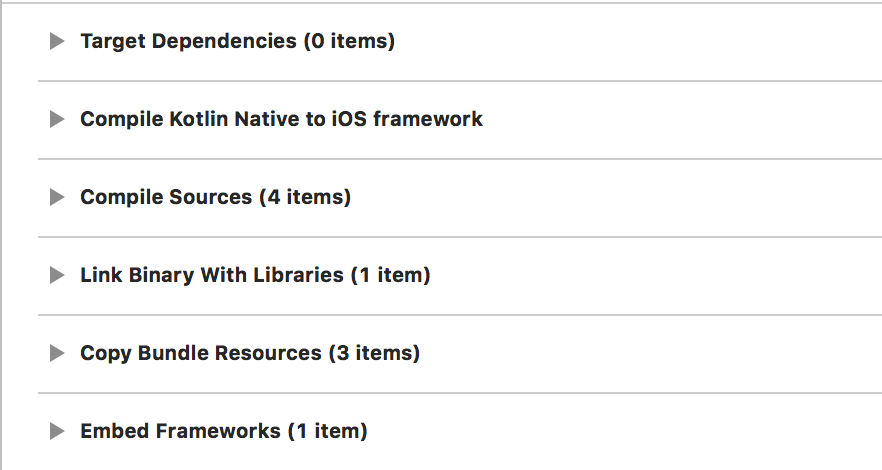
\includegraphics[width=0.75\textwidth]{img/stap6-phases.png}
	\caption{iOS build phases}
	\label{fig:stap6-phases}
\end{figure}

In deze nieuwe build phase moet er een script, afkomstig van \textcite{AlbertGao}, worden toegevoegd: 
\begin{lstlisting}
case "$PLATFORM_NAME" in iphoneos)
NAME=iphone;; iphonesimulator)
NAME=iphone_sim;; *)
echo "Unknown platform: $PLATFORN_NAME"
exit 1;;
esac

"$SRCROOT/../gradlew" -p "$SRCROOT/../platforms/ios" "build"
rm -rf "$SRCROOT/build/"
mkdir "$SRCROOT/build/"
cp -a "$SRCROOT/../platforms/ios/build/konan/bin/$NAME/" "$SRCROOT/build/"
\end{lstlisting}

Bij iedere gradle build van het Kotlin/Native project zal de build.gradle in de platforms/ios map ervoor zorgen dat de Kotlin code omgezet wordt naar een iOS framework. Dit framework vindt men terug in een submap van de build map (platforms/ios/build/). Zie figuur \ref{fig:stap6-build}. Er wordt dus zowel voor een echt toestel (iphone map) als voor een simulator (iphone\char`_sim map) een framework gegenereerd. Dit wordt gedaan omdat beiden op verschillende architecturen worden uitgevoerd.

\begin{figure} [ht]
	\centering
	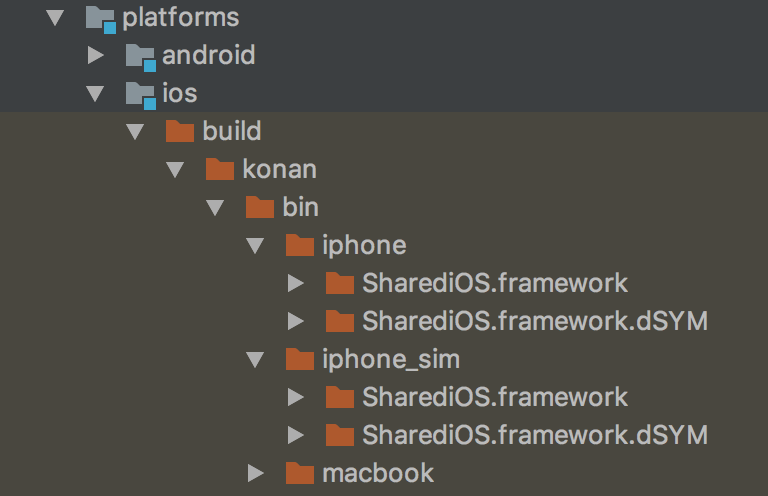
\includegraphics[width=0.60\textwidth]{img/stap6-build.png}
	\caption{iOS build map}
	\label{fig:stap6-build}
\end{figure}

In bovenstaand build phase script wordt gekeken welk type toestel er wordt gebruikt, een echte iPhone of een simulator. Daarna zal het juiste framework gekopieerd worden naar de build folder in de map van je Xcode project. Bij iedere build en/of run van het Xcode project zal bovenstaand script worden uitgevoerd. Dit zal er voor zorgen dat steeds het laatst gegenereerde framework gebruikt zal worden door je Xcode project.

Tenslotte zal het framework nog in de build phases 'Link Binary With Libraries' en 'Embed Frameworks' moeten worden toegevoegd. Hierbij wordt er gelinkt naar het gekopieerde framework in de build folder van je Xcode project.

\section{Aanspreken van code}
\subsection{Android}
Om gebruik te kunnen maken van de Kotlin code in het Android project moet men simpelweg volgende import toevoegen om alle klassen te kunnen gebruiken: 

\begin{lstlisting}
import ilias.vw.libs.*
\end{lstlisting}

\subsection{iOS}
Om gebruik te kunnen maken van het SharediOS framework in de ViewControllers moet het framework worden geimporteerd door bovenaan in de ViewController volgende lijn toe te voegen:

\begin{lstlisting}
import SharediOS
\end{lstlisting}

Het aanmaken van een object in iOS is nu heel simpel geworden. Zoals te zien is in onderstaande code heeft Kotlin/Native een prefix gegeven aan de klassen. Kotlin/Native zal steeds de hoofdletters uit de naam van het framework filteren, dat gekozen wordt in de build.gradle van de iOS folder, zie sectie \ref{sec:ios-build-gradle}. Stel dat het framework KotlinNativeFramework heet, dan zal de prefix KNF zijn en zal de product klasse KNFProduct heten.

\begin{lstlisting}
var product: SOSProduct = SOSProduct(name: "Playstation 4", price: 399.95, description: "Playstation 4 gaming console", productImage: "ps4")
\end{lstlisting}

\section{User interfaces}
De user interface moet dus per platform opgebouwd worden. Er is geen manier om één user interface te ontwikkelen voor beide platformen zoals bijvoorbeeld bij React/Native of Ionic. Dit kan zowel positief als negatief zijn. Het vraagt dubbel zoveel werk maar het geeft wel de mogelijkheid om verschillende accenten te leggen in de user interface per platform.

\section{Optioneel: testen}
\label{sec:testing}
Een essentieel deel van object-oriented programming is het testen van je code. In het Kotlin/Native framework is het mogelijk om je aangemaakte klassen te testen. Zo is er de mogelijkheid om in de common map en per platform een test map toe te voegen. Een voorbeeld van een testklasse:

\begin{lstlisting}
package ilias.vw.libs

import kotlin.test.*

class TestSampleCommon {
 @Test
 fun testCheckChartName() {
  val sample = Cart("test")
  val name = sample.name
  assertEquals(name, "test")
 }
}

\end{lstlisting}

Hierbij wordt er een cart aangemaakt met een naam 'test'. Daarna wordt de naam terug opgevraagd en wordt er gekeken of de naam die we initieel hebben meegegeven effectief gelijk is aan 'test'.

\section{Proof-of-concept}
Screenshots van de schermen van de proof-of-concept.
\subsection{Android}
\begin{figure}[H]
	\centering
	\begin{subfigure}{.5\textwidth}
		\centering
		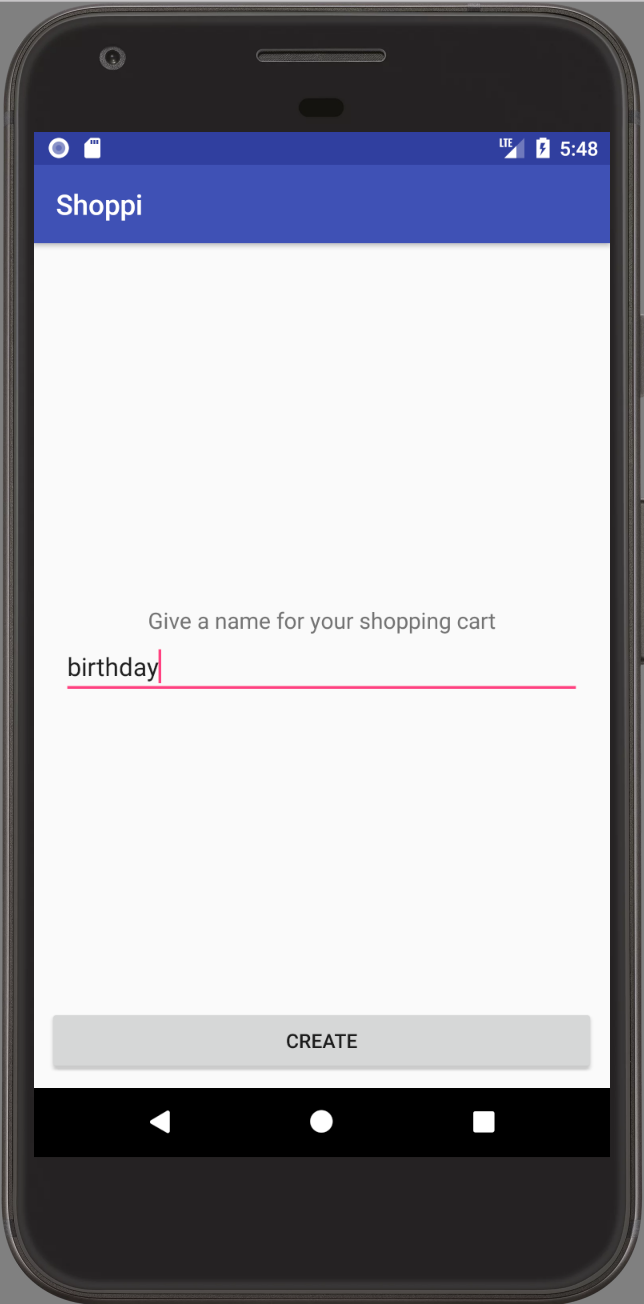
\includegraphics[width=0.65\linewidth]{img/poc/android/1.png}
		\caption{Aanmaken van een shopping cart}
	\end{subfigure}%
	\begin{subfigure}{.5\textwidth}
		\centering
		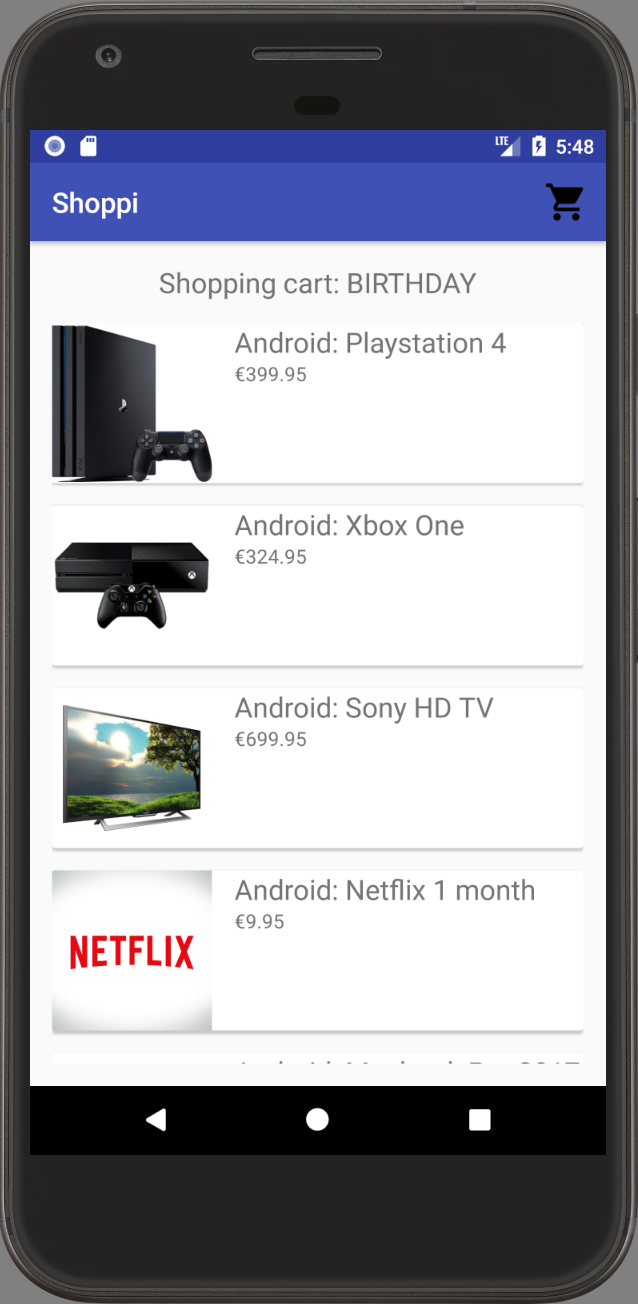
\includegraphics[width=0.65\linewidth]{img/poc/android/2.png}
		\caption{Overzicht van producten}
		\label{fig:sub2}
	\end{subfigure}
\begin{subfigure}{.5\textwidth}
	\centering
	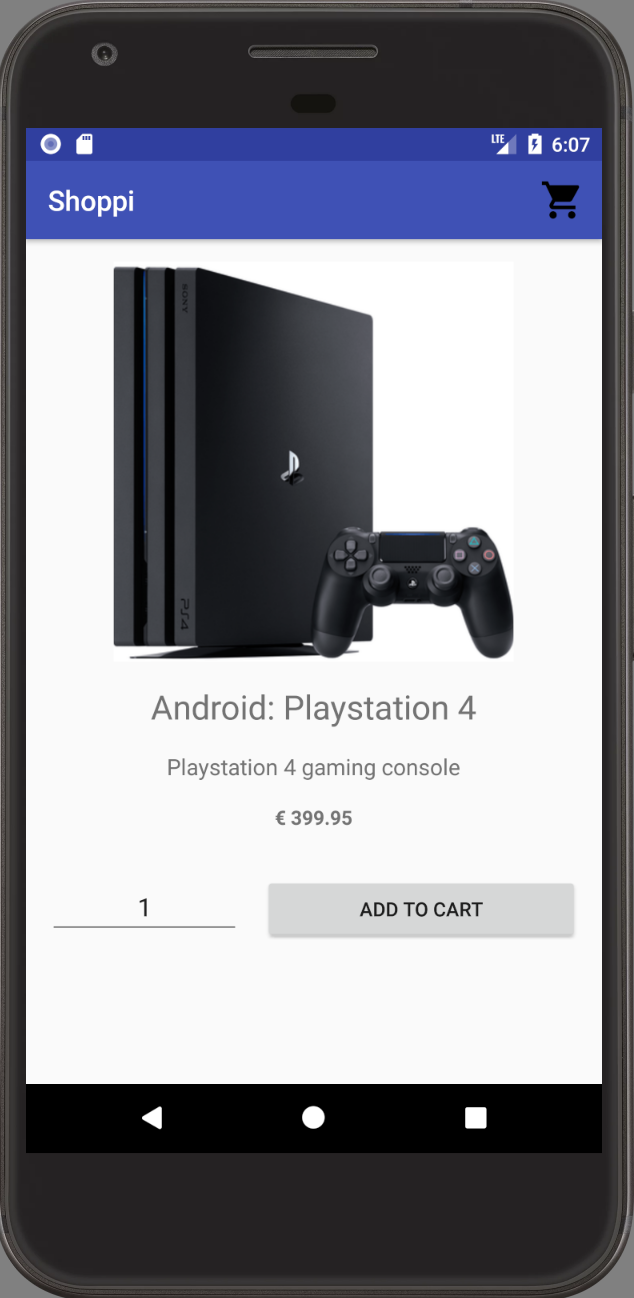
\includegraphics[width=0.65\linewidth]{img/poc/android/3.png}
	\caption{Details van een product}
	\label{fig:sub1}
\end{subfigure}%
\begin{subfigure}{.5\textwidth}
	\centering
	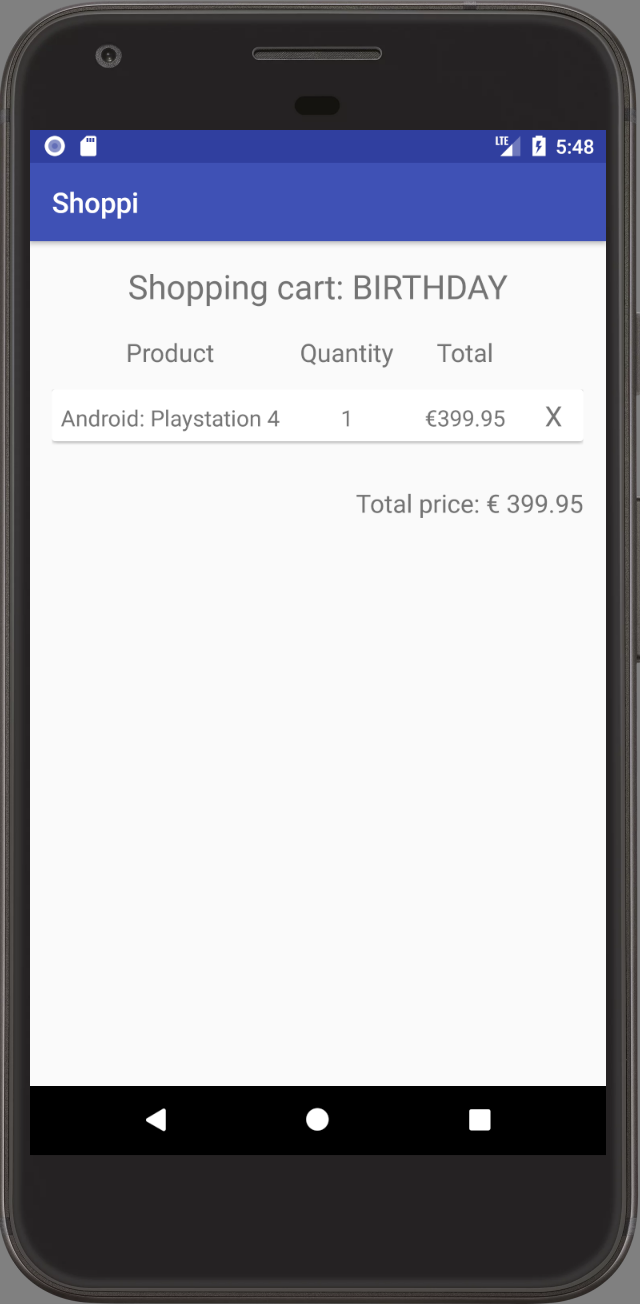
\includegraphics[width=0.65\linewidth]{img/poc/android/4.png}
	\caption{Overzicht winkelmand}
	\label{fig:sub2}
\end{subfigure}
	\caption{Screenshots Android}
	\label{fig:test}
\end{figure}

\subsection{iOS}
\begin{figure}[H]
	\centering
	\begin{subfigure}{.5\textwidth}
		\centering
		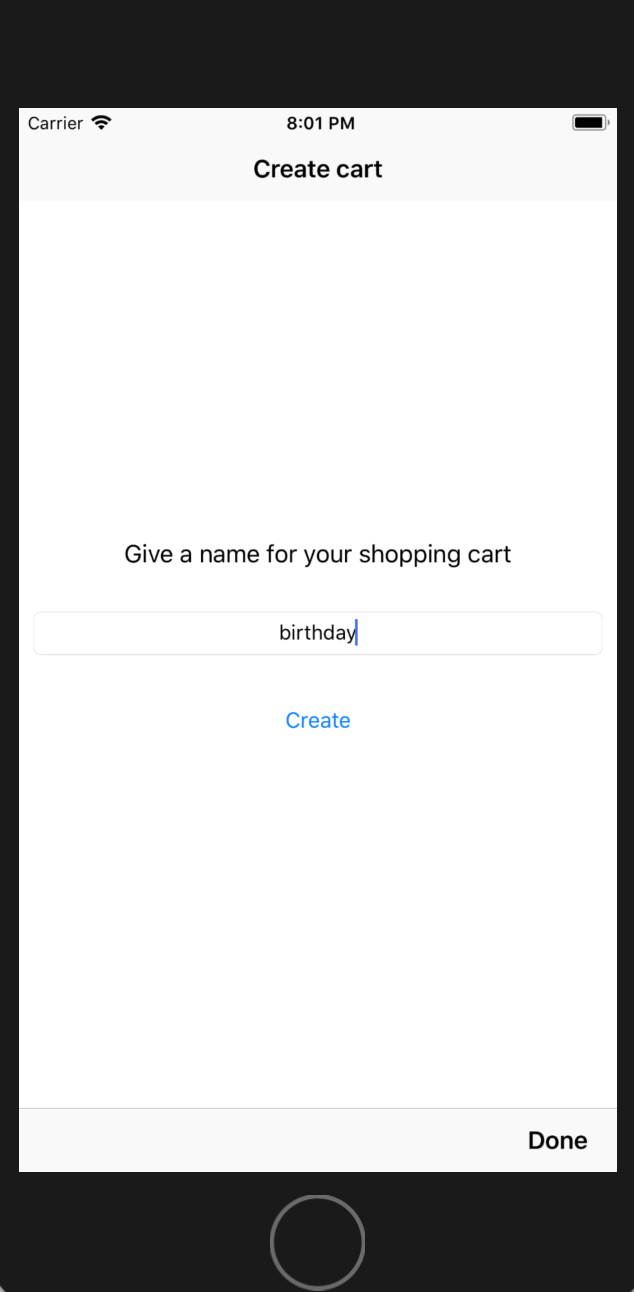
\includegraphics[width=0.65\linewidth]{img/poc/ios/1.png}
		\caption{Aanmaken van een shopping cart}
	\end{subfigure}%
	\begin{subfigure}{.5\textwidth}
		\centering
		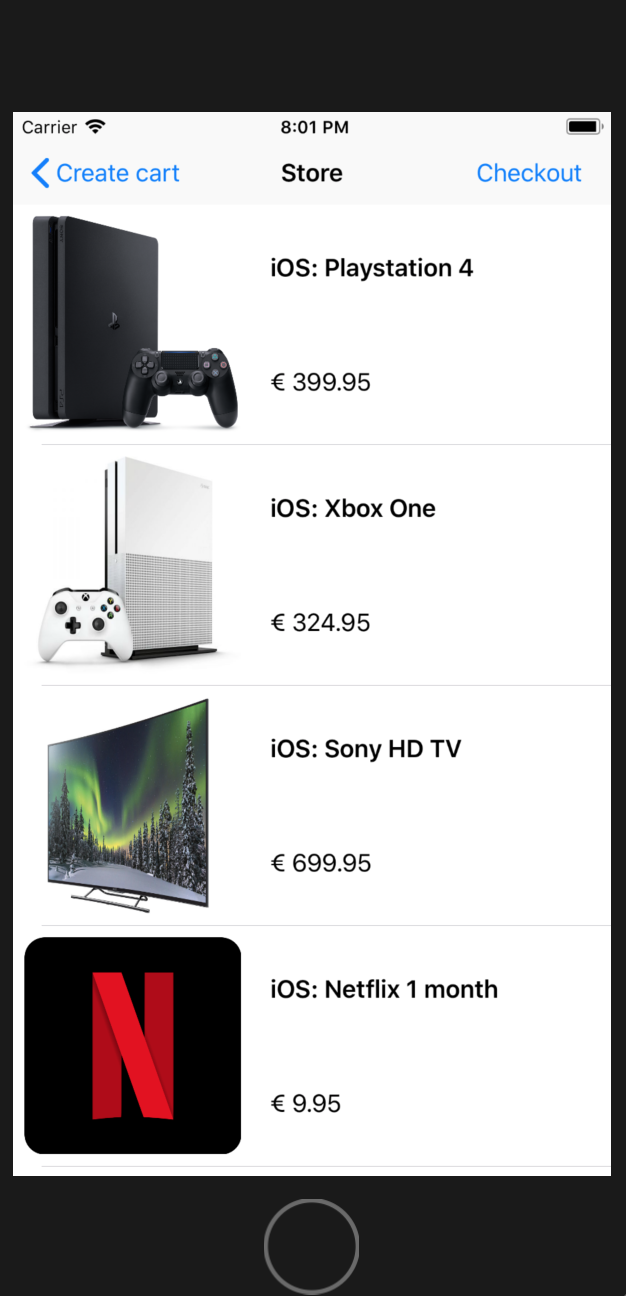
\includegraphics[width=0.65\linewidth]{img/poc/ios/2.png}
		\caption{Overzicht van producten}
		\label{fig:sub2}
	\end{subfigure}
	\begin{subfigure}{.5\textwidth}
		\centering
		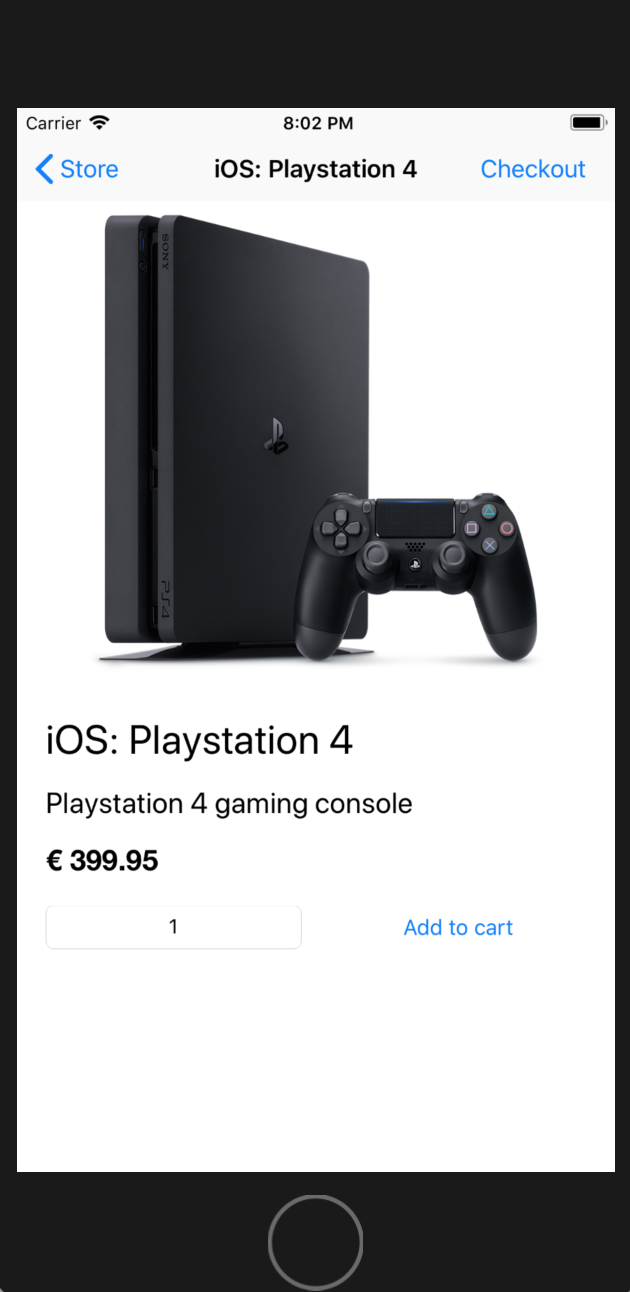
\includegraphics[width=0.65\linewidth]{img/poc/ios/3.png}
		\caption{Details van een product}
		\label{fig:sub1}
	\end{subfigure}%
	\begin{subfigure}{.5\textwidth}
		\centering
		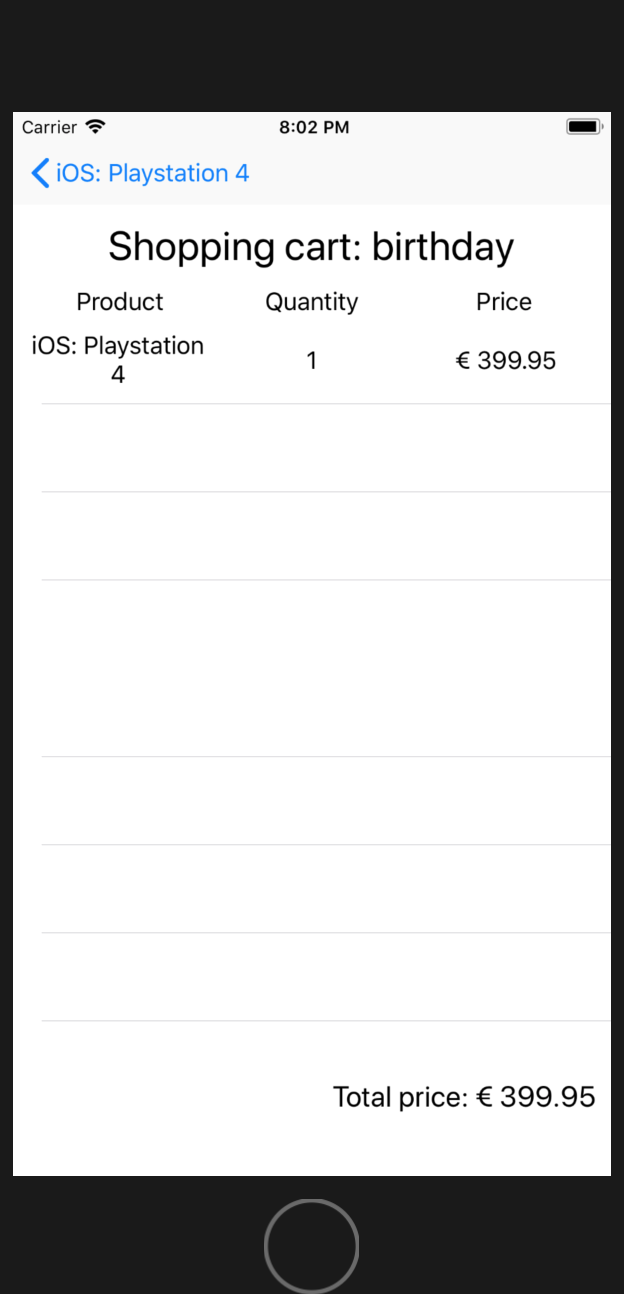
\includegraphics[width=0.65\linewidth]{img/poc/ios/4.png}
		\caption{Overzicht winkelmand}
		\label{fig:sub2}
	\end{subfigure}
	\caption{Screenshots iOS}
	\label{fig:test}
\end{figure}
%...

%%=============================================================================
%% Conclusie
%%=============================================================================

\chapter{Conclusie}
\label{ch:conclusie}

%% TODO: Trek een duidelijke conclusie, in de vorm van een antwoord op de
%% onderzoeksvra(a)g(en). Wat was jouw bijdrage aan het onderzoeksdomein en
%% hoe biedt dit meerwaarde aan het vakgebied/doelgroep? Reflecteer kritisch
%% over het resultaat. Had je deze uitkomst verwacht? Zijn er zaken die nog
%% niet duidelijk zijn? Heeft het onderzoek geleid tot nieuwe vragen die
%% uitnodigen tot verder onderzoek?

\lipsum[76-80]



%%=============================================================================
%% Bijlagen
%%=============================================================================

\appendix

%%---------- Onderzoeksvoorstel -----------------------------------------------

\chapter{Onderzoeksvoorstel}

Het onderwerp van deze bachelorproef is gebaseerd op een onderzoeksvoorstel dat vooraf werd beoordeeld door de promotor. Dat voorstel is opgenomen in deze bijlage.

% Verwijzing naar het bestand met de inhoud van het onderzoeksvoorstel
	\section{Introductie} % The \section*{} command stops section numbering
	\label{sec:introductie}
	%Hier introduceer je werk. Je hoeft hier nog niet te technisch te gaan.
	%
	%Je beschrijft zeker:
	%
	%\begin{itemize}
	%	\item de probleemstelling en context
	%	\item de motivatie en relevantie voor het onderzoek
	%	\item de doelstelling en onderzoeksvraag/-vragen
	%\end{itemize}
	
	Maar wat betekent nu cross-platform? Met cross-platform bedoelt men een systeem/software dat op verschillende platformen en/of besturingssystemen kan draaien. Er zijn al heel wat cross-platform frameworks op de markt. Denk maar aan Xamarin, React Native, Angular in combinatie met het Ionic framework. Momenteel is JetBrains bezig met het ontwikkelen van Kotlin Native waarmee het zou mogelijk zijn om zowel voor web, dekstop als voor mobile (Android, iOS) te ontwikkelen.
	\newline
	\newline
	Kotlin is voor vele programmeurs nieuw. Sinds dit jaar biedt Google volledige ondersteuning voor het gebruik van Kotlin bij Android applicatieontwikkeling. Maar het gaat nog veel verder. JetBrains, de ontwikkelaars van Kotlin, werkt momenteel aan Kotlin Native, het framework dat moet zorgen voor cross-platform ontwikkeling. Maar Kotlin Native is nog heel jong. De huige versie is 0.6 en er bestaat nog maar weinig documentatie rond Kotlin Native. Het probleem echter bij dit framework is dus momenteel dat er heel weinig documentatie en programmeurs dus zelf moeten ontdekken hoe alles momenteel werkt. Dit kan via conferences, voorbeeldprojecten of youtube (kanaal van JetBrains). Maar wat zijn nu de mogelijkheden van Kotlin Native? Zijn er beperkingen? Hoe wordt de GUI opgebouwd? Hoe werkt LLVM, de compiler die alle code omzet naar machinetaal die op elk platform en/of besturingssysteem kan draaien en dus zonder het gebruik van de Java Virtual Machine?
	
	%---------- Stand van zaken ---------------------------------------------------
	
	\section{State-of-the-art}
	\label{sec:state-of-the-art}
	Kotlin, de nieuwe programmeertaal. In 2011 voor het eerst aangekondigd door JetBrains. Zes jaar later biedt Google volledige ondersteuning voor Android applicatieontwikkeling. De voorbije jaren was er nog maar weinig bekend rond Kotlin. Er waren zo goed als geen boeken of andere literatuur op de markt. Hier is het laatste jaar verandering in gekomen. Er worden steeds meer en meer boeken geplubliceerd. 
	\newline
	\newline
	Op het internet zijn er reeds enkele reviews, onderzoeken en boeken beschikbaar. Hierin wordt er verteld waarom men juist wel of niet voor Kotlin moet kiezen. Zo vindt je her en der ook wel eens een vergelijkende studie tussen Java en Kotlin, maar meestal zijn deze niet zo sterk uitgewerkt.
	\newline
	\newline
	Echter is er op het internet een studie beschikbaar \autocite{Pros}, die aangeeft waarom programmeurs Kotlin écht moeten gebruiken. Hieruit blijkt dat Kotlin volledig compatibel zou zijn met Java. Bestaande projecten die geschreven zijn in Java, kunnen dus zonder enig probleem verdergezet worden in Kotlin, dit noemt men de automigration. Bestaande Java frameworks kan men verder gebruiken indien men wenst te programmeren in Kotlin. De taal zou makkelijk te begrijpen zijn voor iedereen die ervaring heeft met OOP (Object-Oriented Programming). Volgens ontwikkelaars die ervaring hebben met Swift 4 zou Kotlin bijna een kopie zijn van Swift 4. Voorbeelden hiervan zijn: geen puntkomma's om de regels af te sluiten en declaratie van variabelen gebeurd op identieke manier.
	\begin{lstlisting}
	var number: Integer = 5
	var text: String = "text"
	\end{lstlisting}
	Bovenstaande code toont beide voorbeelden aan.
	\newline
	\newline
	Een andere studie \autocite{Cons}, beschrijft dan de nadelen van Kotlin. Kotlin zou geen gebruik maken van namespaces. De static modifier zou verdwenen zijn, maar een alternatieve manier is dan weer mogelijk via @JvmField. Het compileren van projecten in Android Studio zou veel tijd in beslag nemen en het gebruik van annotations zou nog niet volledig geoptimaliseerd zijn. Zo blijkt dat er toch nog wat werk is aan Kotlin. We zitten dan ook nog maar aan versie 1.2. 
	\newline
	\newline
	Wat betreft het gebruik van Kotlin als cross-platform programmeertaal \autocite{dzone}, wordt er sterk gewerkt aan Kotlin Native. Momenteel is dit nog in development, JetBrains zelf biedt reeds enkele projecten aan waar ontwikkelaars met de slag kunnen. Zo geven ze de programmeurs de mogelijkheid om reeds kennis te maken met de werking van Kotlin Native ook al is er nog geen documentatie over dit framework. Er is echter ook een kleine tutorial op de website van JetBrains aanwezig om een simpele applicatie te bouwen die 'Hello World' op het scherm print.
	\newline
	\newline
	Op het internet zijn er voldoende bronnen te vinden om applicaties te bouwen met Kotlin voor één platform. Dit kan gaan over een webapplicatie die gebruik maakt van het Spring framework, waarbij Spring gebruik maakt van de taalfeatures van Kotlin. Wat Android betreft kan men gewoon in Android Studio een applicatie geschreven in Android converteren naar Kotlin. Tenslotte is er de mogelijkheid om voor een desktopapplicatie, KotlinFX te gebruiken. KotlinFX is een library die dezelfde functionaliteit biedt als JavaFX, een library om interfaces te bouwen.
	\newline
	\newline
	Zoals te lezen is, is er op het internet voldoende informatie te vinden om applicaties te bouwen voor één platform. Maar is het nu ook mogelijk om via één codebase verschillende platformen aan te spreken? Kan je door het eenmalig schrijven van code, een applicatie ontwikkelen die zowel op Android als op iOS kan draaien? Dit is het grote verschil met mijn onderzoek.
	
	% Voor literatuurverwijzingen zijn er twee belangrijke commando's:
	% \autocite{KEY} => (Auteur, jaartal) Gebruik dit als de naam van de auteur
	%   geen onderdeel is van de zin.
	% \textcite{KEY} => Auteur (jaartal)  Gebruik dit als de auteursnaam wel een
	%   functie heeft in de zin (bv. ``Uit onderzoek door Doll & Hill (1954) bleek
	%   ...'')
	
	%Je mag gerust gebruik maken van subsecties in dit onderdeel.
	
	%---------- Methodologie ------------------------------------------------------
	\section{Methodologie}
	\label{sec:methodologie}
	Vooraleer er aan de slag wordt gegaan met het uittesten van Kotlin Native, of het analyseren van voorbeeldprojecten van JetBrains, is het belangrijk om te onderzoeken hoe het nu komt dat Kotlin Native op verschillende platformen kan draaien. Kotlin is oorspronkelijk, net zoals Java, een programmeertaal die gebruik maakt van de Java Virtual Machine. Het zal daarom dus belangrijk zijn om te onderzoeken waarop Kotlin Native draait, wat de taak is van de LLVM compiler. Dit zal gebeuren aan de hand van een literatuurstudie.
	\newline
	\newline
	Daarna worden de voorbeeldprojecten van JetBrains, geschreven in Kotlin Native, geanalyseerd om de werking van Kotlin Native te achterhalen. De bedoeling is om te kijken naar bepaalde aspecten. Hoe wordt de user interface opgebouwd, wordt er per platform een UI opgebouwd of is er slechts één UI? Hoe kunnen specifieke native modules gebruikt worden? 
	\newline
	\newline
	Eenmaal de werking van Kotlin Native duidelijk is en voldoende gedocumenteerd is, is het het doel om zelf aan de slag te gaan met Kotlin Native en een kleine cross-platform applicatie te schrijven.
	
	%---------- Verwachte resultaten ----------------------------------------------
	\section{Verwachte resultaten}
	\label{sec:verwachte_resultaten}
	Ten eerste wordt verwacht om uit de literatuurstudie te kunnen besluiten wat de werking is van de LLVM compiler. Hierdoor is het duidelijk hoe Kotlin Native er voor zorgt dat Kotlin voor verschillende platformen kan gebruikt worden.
	\newline
	\newline
	Anderzijds wordt een zeer duidelijke documentatie verwacht over de werking van Kotlin Native zodat mensen die geïnteresseerd zijn om Kotlin Native in de toekomst te gebruiken deze documentatie kunnen gebruiken. 
	
	%---------- Verwachte conclusies ----------------------------------------------
	\section{Verwachte conclusies}
	\label{sec:verwachte_conclusies}
	Uit dit onderzoek verwacht ik te kunnen concluderen dat Kotlin meer dan geschikt is als cross-platform programmeertaal. Dit aangezien Kotlin volledig ondersteund wordt door Google wat betreft de ontwikkeling van Android applicaties. Er wordt nog steeds verder gebouwd aan Kotlin Native. Maar natuurlijk, Kotlin is een nieuwe taal, waar nog veel aan gesleuteld zal moeten worden. De toekomst ziet er enkel maar veel belovend uit. De kans is groot dat een groot aantal programmeurs zal overschakelen naar deze taal. Kotlin heeft zeker en vast de kracht om programmeurs, die al jaren in dit vak zitten en zich hebben vastgehecht aan een bepaalde programmeertaal, mee te slepen in het Kotlin-avontuur. Ook voor Swift programmeurs zal de aanpassing naar Kotlin niet groot zijn wegens de grote gelijkenissen tussen de twee programmeertalen.
	
	%------------------------------------------------------------------------------
	% Referentielijst
	%------------------------------------------------------------------------------
	% TODO: de gerefereerde werken moeten in BibTeX-bestand ``biblio.bib''
	% voorkomen. Gebruik JabRef om je bibliografie bij te houden en vergeet niet
	% om compatibiliteit met Biber/BibLaTeX aan te zetten (File > Switch to
	% BibLaTeX mode)



%%---------- Andere bijlagen --------------------------------------------------
% TODO: Voeg hier eventuele andere bijlagen toe
%\input{...}

%%---------- Referentielijst --------------------------------------------------
\nocite{*}
\printbibliography[heading=bibintoc]

%\addcontentsline{toc}{chapter}{\textcolor{maincolor}{\IfLanguageName{dutch}{Bibliografie}{Bibliography}}}

\end{document}
